
% IUT-Thesis v2.5
%CHANGE LOG IUT-Thesis v2.5
%---------------------------
%- Add some options to signature pages
%- Adaption to Texlive 2016, Xeperian 18.2 and Bidi 30.2
%- Fix some buges: paragraph footnote, reference style, and ...


% این قالب بر اساس فرمت پایان‌نامه‌ها و رساله‌های تحصیلات تکمیلی دانشگاه صنعتی اصفهان تهیه شده است. شما می‌توانید آخرین نسخه این قالب را از دریافت کنید.

% توصیه می‌شود که از توزیع تک‌لایو (TexLive) استفاده شود:
% http://tug.org/texlive/acquire-iso.html

% موفق باشید.
% محمد جان‌نثاری
% mohammad.jannesari@gmail.com
% امین فخاری
% a101.fakhari@gmail.com
% ‌فروردین 1396
% -----------------------------------------------------------------------------------

% نکات:

% برای دریافت نتیجه مطلوب از این قالب بایستی از آخرین نسخه تک‌لایو به همراه Xepersian نسخه 18.2 , Bidi نسخه 30.2 استفاده شود.

% برای آن‌که پردازش فایل و مشاهده خروجی در هنگام نوشتن پایان‌نامه آسان‌تر و سریع‌تر انجام شود، انجام موارد زیر توصیه می گردد:
% الف) فصل‌ها و بخش‌هایی که در حال نوشتن آن‌ها نیستید را غیر فعال کنید. به‌عنوان مثال، در این قالب، این دستورات را می‌توان در صورت عدم نیاز با اضافه کردن % به طور موقت غیرفعال کرد:
% \MakeTitlePage
% \MakeFarsiSignaturePage
% \clearpage
\thispagestyle{empty}
\newgeometry{left=3cm,right=4cm,top=7cm}

{\BZarScaleOne
{\fontsize{20pt}{0}\selectfont
\noindent
% عنوان تشکر و قدردانی---------------------------------------------------------
تشکر و قدردانی
% ؛---------------------------------------------------------
}}
\vspace{0.5cm}

{\BZarScaleOne
{\fontsize{12pt}{0.9cm}\selectfont % Zar 13
\noindent
% متن تشکر و قدردانی---------------------------------------------------------
سپاس خدای را که سخنوران، در ستودن او بمانند ...
% ؛---------------------------------------------------------
}}

\restoregeometry
% \MakeCopyRightPage
% \clearpage
\thispagestyle{empty}
\newgeometry{left=3cm,right=4cm,top=7cm}

{\BZarScaleOne
{\fontsize{28pt}{0}\selectfont
\noindent
% تقدیم اثر---------------------------------------------------------
{\normalsize تقدیم به}
\\[1cm]
\hspace*{1cm}
\centering{\textbf{\IrNasScaleOne\fontsize{54pt}{0}\selectfont ...}}
% ؛---------------------------------------------------------
}}
		
\restoregeometry
% \MakeTableOfContents
% \MakeListOfFigures
% \MakeListOfTables
% \MakeFarsiAbstract
% \input{Chapters/Chapter#}
% \MakeAppendices
% \section{مدیریت مراجع در لاتک}\label{App:RefMan}
در بخش \ref{Sec:Ref} اشاره شد که با دستور 
 \lr{\textbackslash bibitem}
  می‌توان یک مرجع را تعریف نمود و با فرمان
 \lr{\textbackslash cite}
  به آن ارجاع داد. این روش برای تعداد مراجع زیاد و تغییرات آنها مناسب نیست. در ادامه به صورت مختصر توضیحی در خصوص برنامه \lr{BibTeX} که همراه با توزیع‌های معروف تِک عرضه می‌شود و نحوه استفاده از آن در زی‌پرشین خواهیم داشت.

\subsection{ مدیریت مراجع با  \texorpdfstring{\lr{Bib\TeX}}{Bib\TeX} }
یکی از روش‌های قدرتمند و انعطاف‌پذیر برای نوشتن مراجع مقالات و مدیریت مراجع در لاتک، استفاده از  \lr{BibTeX} است.
 روش کار با  \lr{BibTeX} به این صورت است که مجموعه‌ی همه‌ی مراجعی را که در پروژه/پایان‌نامه/رساله استفاده کرده یا خواهیم کرد، 
در پرونده‌ی جداگانه‌ای نوشته و به آن فایل در سند خودمان به صورت مناسب لینک می‌دهیم.
 کنفرانس‌ها یا مجله‌های گوناگون برای نوشتن مراجع، قالب‌ها یا قراردادهای متفاوتی دارند که به آنها استیلهای مراجع گفته می‌شود.
 در این حالت به کمک ‌استیل‌های \lr{BibTeX} خواهید توانست تنها با تغییر یک پارامتر در پرونده‌ی ورودی خود، مراجع را مطابق قالب موردنظر تنظیم کنید. 
 بیشتر مجلات و کنفرانس‌های معتبر یک پرونده‌ی سبک (\lr{BibTeX Style}) با پسوند \lr{bst} در وب‌گاه خود می‌گذارند که برای همین منظور طراحی شده است.

به جز نوشتن مقالات این سبک‌ها کمک بسیار خوبی برای تهیه‌ی مستندات علمی همچون پایان‌نامه‌هاست که فرد می‌تواند هر قسمت از کارش را که نوشت مراجع مربوطه را به بانک مراجع خود اضافه نماید. با داشتن چنین بانکی از مراجع، وی خواهد توانست به راحتی یک یا چند ارجاع به مراجع و یا یک یا چند بخش را حذف یا اضافه ‌نماید؛ 
مراجع به صورت خودکار مرتب شده و فقط مراجع ارجاع داده شده در قسمت کتاب‌نامه خواهندآمد. قالب مراجع به صورت یکدست مطابق سبک داده شده بوده و نیازی نیست که کاربر درگیر قالب‌دهی به مراجع باشد. 
در این جا مجموعه‌ سبک‌های بسته \lr{Persian-bib} که برای  زی‌پرشین آماده شده‌اند به صورت مختصر معرفی شده و روش کار با آن‌ها گفته می‌شود. برای اطلاع بیشتر به راهنمای بسته‌ی \lr{Persian-bib} مراجعه فرمایید.
\subsection{سبک‌های فعلی قابل استفاده در زی‌پرشین}
در حال حاضر فایلهای سبک زیر برای استفاده در زی‌پرشین آماده شده‌اند:

\singlespacing
\begin{description}
\item [\lr{unsrt-fa.bst}] این سبک متناظر با \lr{unsrt.bst} می‌باشد. مراجع به ترتیب ارجاع در متن ظاهر می‌شوند.
\item [\lr{plain-fa.bst}] این سبک متناظر با \lr{plain.bst} می‌باشد. مراجع بر اساس نام‌خانوادگی نویسندگان، به ترتیب صعودی مرتب می‌شوند.
 همچنین ابتدا مراجع فارسی و سپس مراجع انگلیسی خواهند آمد.
\item [\lr{acm-fa.bst}] این سبک متناظر با \lr{acm.bst} می‌باشد. شبیه \lr{plain-fa.bst} است.  قالب مراجع کمی متفاوت است. اسامی نویسندگان انگلیسی با حروف بزرگ انگلیسی نمایش داده می‌شوند. (مراجع مرتب می‌شوند)
\item [\lr{ieeetr-fa.bst}] این سبک متناظر با \lr{ieeetr.bst} می‌باشد. (مراجع مرتب نمی‌شوند)
\item [\lr{plainnat-fa.bst}] این سبک متناظر با \lr{plainnat.bst} می‌باشد. نیاز به بسته \lr{natbib} دارد. (مراجع مرتب می‌شوند)
\item [\lr{chicago-fa.bst}] این سبک متناظر با \lr{chicago.bst} می‌باشد. نیاز به بسته \lr{natbib} دارد. (مراجع مرتب می‌شوند)
\item [\lr{asa-fa.bst}] این سبک متناظر با \lr{asa.bst} می‌باشد. نیاز به بسته \lr{natbib} دارد. (مراجع مرتب می‌شوند)
\item[\lr{ModifiedIEEEtranFa.bst}] این سبک متناظر با نحوه ارجاع در پایان‌نامه‌های دانشگاه صنعتی اصفهان می‌باشد.
\end{description}
\doublespacing

با استفاده از استیلهای فوق می‌توانید به انواع مختلفی از مراجع فارسی و لاتین ارجاع دهید. به عنوان نمونه مرجع 
\cite{Omidali82phdThesis}
 یک نمونه پروژه دکترا (به فارسی) و مرجع 
\cite{Vahedi87} یک نمونه مقاله مجله فارسی است.
مرجع 
\cite{Amintoosi87afzayesh}  یک نمونه  مقاله کنفرانس فارسی و
مرجع 
\cite{Pedram80osool} یک نمونه کتاب فارسی با ذکر مترجمان و ویراستاران فارسی است. مرجع 
\cite{Khalighi07MscThesis} یک نمونه پروژه کارشناسی ارشد انگلیسی و
\cite{Khalighi87xepersian} هم یک نمونه متفرقه  می‌باشند.
مراجع 
\cite{Gonzalez02book,Baker02limits} 
نمونه کتاب و مقاله انگلیسی هستند.

استیل مورد استفاده در این پروژه/پایان‌نامه/رساله 
\lr{ModifiedIEEEtranFa}
است که خروجی آنرا در بخش مراجع می‌توانید مشاهده کنید.
نمونه  خروجی سبک \lr{asa-fa} در شکل \ref{fig:asafa} آمده است.

\begin{figure}[t]
\centering
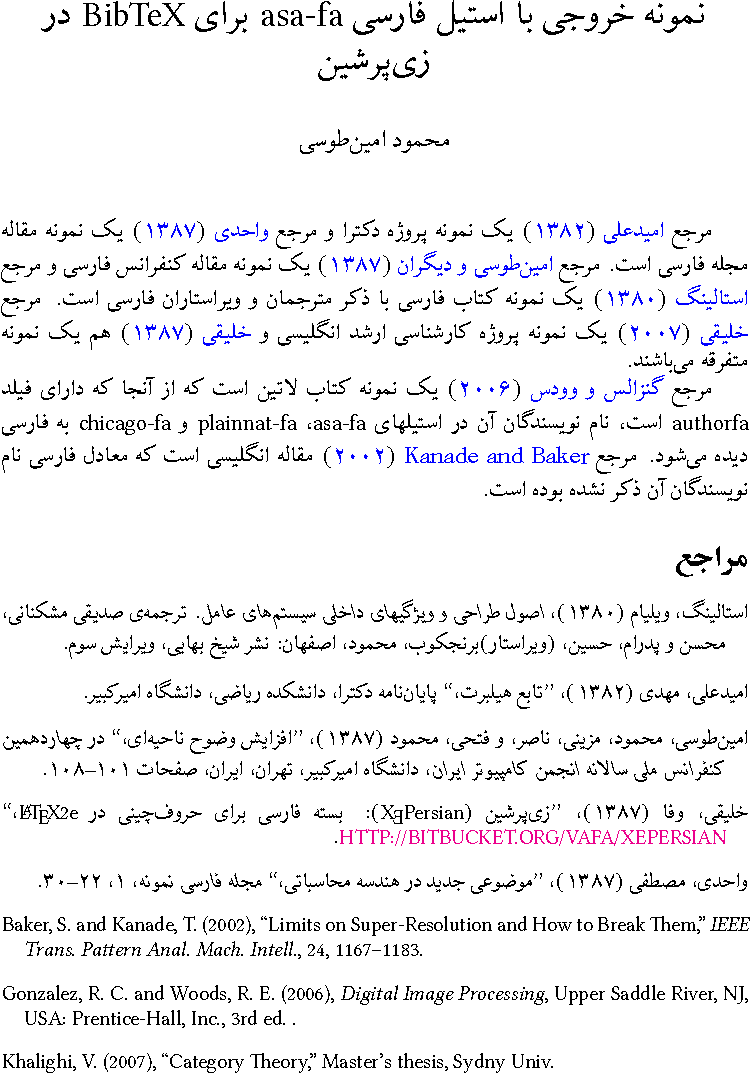
\includegraphics[width=.8\textwidth]{Figures/App1/asa-fa-crop.pdf}
\caption{نمونه خروجی با سبک \lr{asa-fa}}
\label{fig:asafa}
\end{figure} 
\subsection{ نحوه استفاده از سبک‌های فارسی}
برای استفاده از بیب‌تک باید مراجع خود را در یک فایل با پسوند \lr{bib} ذخیره نمایید. یک فایل \lr{bib} در واقع یک پایگاه داده از مراجع\LTRfootnote{Bibliography Database}  شماست که هر مرجع در آن به عنوان یک رکورد از این پایگاه داده
با قالبی خاص ذخیره می‌شود. به هر رکورد یک مدخل\LTRfootnote{Entry} گفته می‌شود. یک نمونه مدخل برای معرفی کتاب \lr{Digital Image Processing} در ادامه آمده است:

\singlespacing
\begin{LTR}
\begin{verbatim}
@BOOK{Gonzalez02image,
  AUTHOR =      {Rafael Gonzalez and Richard Woods},
  TITLE =       {Digital Image Processing},
  PUBLISHER =   {Prentice-Hall, Inc.},
  YEAR =        {2006},
  EDITION =     {3rd},
  ADDRESS =     {Upper Saddle River, NJ, USA}
}
\end{verbatim}
\end{LTR}
\doublespacing

در مثال فوق، \lr{@BOOK} مشخصه‌ی شروع یک مدخل مربوط به یک کتاب و \lr{Gonzalez02book} برچسبی است که به این مرجع منتسب شده است.
 این برچسب بایستی یکتا باشد. برای آنکه فرد به راحتی بتواند برچسب مراجع خود را به خاطر بسپارد و حتی‌الامکان برچسب‌ها متفاوت با هم باشند معمولاً از قوانین خاصی به این منظور استفاده می‌شود. یک قانون می‌تواند فامیل نویسنده‌ی اول+دورقم سال نشر+اولین کلمه‌ی عنوان اثر باشد. به \lr{AUTHOR} و $\dots$ و \lr{ADDRESS} فیلدهای این مدخل گفته می‌شود؛ که هر یک با مقادیر مربوط به مرجع مقدار گرفته‌اند. ترتیب فیلدها مهم نیست. 

انواع متنوعی از مدخل‌ها برای اقسام مختلف مراجع همچون کتاب، مقاله‌ی کنفرانس و مقاله‌ی ژورنال وجود دارد که برخی فیلدهای آنها با هم متفاوت است. 
نام فیلدها بیانگر نوع اطلاعات آن می‌باشد. مثالهای ذکر شده در فایل \lr{References.bib} کمک خوبی به شما خواهد بود. 
%این فایل یک فایل متنی بوده و با ویرایشگرهای معمول همچون \lr{Notepad++} قابل ویرایش می‌باشد. برنامه‌هایی همچون 
%\lr{TeXMaker}
% امکاناتی برای نوشتن این مدخل‌ها دارند و به صورت خودکار فیلدهای مربوطه را در فایل \lr{bib}  شما قرار می‌دهند.  
با استفاده از سبک‌های فارسی آماده شده، محتویات هر فیلد می‌تواند به فارسی نوشته شود، ترتیب مراجع و نحوه‌ی چینش فیلدهای هر مرجع را سبک مورد استفاده  مشخص خواهد کرد.

نکته: بدون اعمال تنظیمات موردنیاز \lr{Bib\TeX} در \lr{TeXWorks}، مراجع فارسی در استیل‌هایی که مراجع را به صورت مرتب شده چاپ می‌کنند، ترتیب کاملاً درستی نخواهند داشت. برای توضیحات بیشتر \cite{persianbib87userguide} را ببینید یا به سایت پارسی‌لاتک مراجعه فرمایید.

\textbf{برای درج مراجع خود لازم نیست نگران موارد فوق باشید. در فایل 
\lr{References.bib}
 که همراه با این پروژه/پایان‌نامه/رساله هست، موارد مختلفی درج شده است و کافیست مراجع خود را جایگزین موارد مندرج در آن نمایید.
}

پس از قرار دادن مراجع خود، یک بار \lr{XeLaTeX} را روی سند خود اجرا نمایید، سپس \lr{bibtex} و پس از آن دوبار \lr{XeLaTeX} را. در \lr{TeXstudio} کلید \lr{F8} و در \lr{TeXWorks} هم گزینه‌ی \lr{BibTeX} از منوی \lr{Typeset}، \lr{BibTeX} را روی سند شما اجرا می‌کنند.

برای بسیاری از مقالات لاتین حتی لازم نیست که مدخل مربوط به آنرا خودتان بنویسید. با جستجوی نام مقاله + کلمه \lr{bibtex}  در اینترنت سایتهای بسیاری همچون \lr{ACM} و \lr{ScienceDirect} را خواهید یافت که مدخل \lr{bibtex} مربوط به مقاله شما را دارند و کافیست آنرا به انتهای فایل \lr{References} اضافه کنید.

از هر یک از سبکهای \lr{Persian-bib} می‌توانید استفاده کنید، البته اگر از سه استیل آخر استفاده می‌کنید و مایلید که مراجع شما شماره بخورند باید بسته \lr{natbib} را با گزینه \lr{numbers} فراخوانی نمایید.
\newpage
\section{‌جدول، نمودار و الگوریتم در لاتک}\label{App:Latex:More}
در این بخش نمونه مثالهایی از جدول، نمودار و الگوریتم در لاتک را خواهیم دید.
\subsection{مدلهای حرکت دوبعدی}
بسیاری از اوقات حرکت بین دو تصویر از یک صحنه با یکی از مدلهای پارامتری ذکر شده در جدول \eqref{tab:MotionModels} قابل مدل نمودن می‌باشد.  
\begin{table}[ht]
	\caption{مدلهای تبدیل.}
	\label{tab:MotionModels}
	\centering
	\onehalfspacing
	\begin{tabular}{|r|c|l|r|}
		\hline نام مدل & درجه آزادی & تبدیل مختصات & توضیح \\ 
		\hline انتقالی & ۲ & $\begin{aligned} x'=x+t_x \\ y'=y+t_y \end{aligned}$  &  انتقال دوبعدی\\ 
		\hline اقلیدسی & ۳ & $\begin{aligned} x'=xcos\theta - ysin\theta+t_x \\ y'=xsin\theta+ycos\theta+t_y \end{aligned}$  &  انتقالی+دوران \\ 
		\hline مشابهت & ۴ & $\begin{aligned} x'=sxcos\theta - sysin\theta+t_x \\ y'=sxsin\theta+sycos\theta+t_y  \end{aligned}$  & اقلیدسی+تغییرمقیاس \\ 
		\hline آفین & ۶ & $\begin{aligned} x'=a_{11}x+a_{12}y+t_x \\ y'=a_{21}x+a_{22}y+t_y \end{aligned}$  & مشابهت+اریب‌شدگی \\ 
		\hline  پروجکتیو & ۸ & $\begin{aligned} x'&=(m_1x+m_2y+m_3)/D \\ y'&=(m_4x+m_5y+m_6)/D \\ D&=m_7x+m_8y+1 \end{aligned}$  & آفین+\lr{keystone+chirping} \\ 
		\hline  شارنوری & $\infty $ & $\begin{aligned} x'=x+v_x(x,y) \\ y'=y+v_y(x,y) \end{aligned}$  &  حرکت آزاد\\ 
		\hline 
	\end{tabular} 
\end{table}

\subsection{ماتریس}

شناخته‌شده‌ترین روش تخمین ماتریس هوموگرافی الگوریتم تبدیل خطی مستقیم (\lr{DLT\LTRfootnote{Direct Linear Transform}}) است.  فرض کنید چهار زوج نقطهٔ متناظر در دو تصویر در دست هستند،  $\mathbf{x}_i\leftrightarrow\mathbf{x}'_i$   و تبدیل با رابطهٔ
$\mathbf{x}'_i = H\mathbf{x}_i$
نشان داده می‌شود که در آن:
\[\mathbf{x}'_i=(x'_i,y'_i,w'_i)^\top  \]
و
\[ H=\left[
\begin{array}{ccc}
h_1 & h_2 & h_3 \\ 
h_4 & h_5 & h_6 \\ 
h_7 & h_8 & h_9
\end{array} 
\right]\]
رابطه زیر را برای الگوریتم  \eqref{alg:DLT} لازم دارم.
\begin{equation}\label{eq:DLT_Ah}
\left[
\begin{array}{ccc}
0^\top & -w'_i\mathbf{x}_i^\top & y'_i\mathbf{x}_i^\top \\ 
w'_i\mathbf{x}_i & 0^\top & -x'_i\mathbf{x}_i^\top \\ 
- y'_i\mathbf{x}_i^\top & x'_i\mathbf{x}_i^\top & 0^\top
\end{array} 
\right]
\left(
\begin{array}{c}
\mathbf{h}^1 \\ 
\mathbf{h}^2 \\ 
\mathbf{h}^3
\end{array} 
\right)=0
\end{equation}

\subsection{الگوریتم با دستورات فارسی}
با مفروضات فوق، الگوریتم \lr{DLT} به صورت نشان داده شده در الگوریتم \eqref{alg:DLT}  خواهد بود.
\begin{algorithm}[t]
	\onehalfspacing
	\caption{الگوریتم \lr{DLT} برای تخمین ماتریس هوموگرافی.} \label{alg:DLT}
	\begin{algorithmic}[1]
		\REQUIRE $n\geq4$ زوج نقطهٔ متناظر در دو تصویر 
		${\mathbf{x}_i\leftrightarrow\mathbf{x}'_i}$،\\
		\ENSURE ماتریس هوموگرافی $H$ به نحوی‌که: 
		$\mathbf{x}'_i = H \mathbf{x}_i$.
		\STATE برای هر زوج نقطهٔ متناظر
		$\mathbf{x}_i\leftrightarrow\mathbf{x}'_i$ 
		ماتریس $\mathbf{A}_i$ را با استفاده از رابطهٔ \ref{eq:DLT_Ah} محاسبه کنید.
		\STATE ماتریس‌های ۹ ستونی  $\mathbf{A}_i$ را در قالب یک ماتریس $\mathbf{A}$ ۹ ستونی ترکیب کنید. 
		\STATE تجزیهٔ مقادیر منفرد \lr{(SVD)}  ماتریس $\mathbf{A}$ را بدست آورید. بردار واحد متناظر با کمترین مقدار منفرد جواب $\mathbf{h}$ خواهد بود.
		\STATE  ماتریس هوموگرافی $H$ با تغییر شکل $\mathbf{h}$ حاصل خواهد شد.
	\end{algorithmic}
\end{algorithm}

\subsection{الگوریتم با دستورات لاتین}
الگوریتم \ref{alg:RANSAC} یک الگوریتم با دستورات لاتین است.

\begin{algorithm}[t]
	\onehalfspacing
	\caption{الگوریتم \lr{RANSAC} برای تخمین ماتریس هوموگرافی.} \label{alg:RANSAC}
	\begin{latin}
		\begin{algorithmic}[1]
			\REQUIRE $n\geq4$ putative correspondences, number of estimations, $N$, distance threshold $T_{dist}$.\\
			\ENSURE Set of inliers and Homography matrix $H$.
			\FOR{$k = 1$ to $N$}
			\STATE Randomly choose 4 correspondence,
			\STATE Check whether these points are colinear, if so, redo the above step
			\STATE Compute the homography $H_{curr}$ by DLT algorithm from the 4 points pairs,
			\STATE $\ldots$ % الگوریتم کامل نیست
			\ENDFOR
			\STATE Refinement: re-estimate H from all the inliers using the DLT algorithm.
		\end{algorithmic}
	\end{latin}
\end{algorithm}

\subsection{نمودار}
لاتک بسته‌هایی با قابلیت‌های زیاد برای رسم انواع مختلف نمودارها دارد. مانند بسته‌های \lr{Tikz} و  \lr{PSTricks}. توضیح اینها فراتر از این پیوست کوچک است. مثالهایی از رسم نمودار را در مجموعه پارسی‌لاتک خواهید یافت. توصیه می‌کنم که حتماً مثالهایی از برخی از آنها را ببینید. راهنمای همه آنها در تک‌لایو هست. نمونه مثالهایی از بسته \lr{Tikz} را می‌توانید در \url{http://www.texample.net/tikz/examples/} ببینید.

\subsection{تصویر}
نمونه تصاویری در بخش قبل دیدیم. دو تصویر شیر کنار هم را هم در شکل \ref{fig:twolion} مشاهده می‌کنید.
\begin{figure}[t]
	\centering 
	\subfloat[شیر ۱]{ \label{fig:twolion:one}
		
\includegraphics[width=.3\textwidth]{Figures/Ch2/lion.jpg}}
	%\hspace{2mm}
	\subfloat[شیر ۲]{ \label{fig:twolion:two}
		
\includegraphics[width=.3\textwidth]{Figures/Ch2/lion.jpg}}
	\caption{دو شیر}
	\label{fig:twolion} %% label for entire figure
\end{figure}
% \MakeEnglishAbstract
% \MakeEnglishSignaturePage
% ب) از گزینه draft برای فراخوانی کلاس استفاده کنید. یعنی
% \documentclass[a4paper,fleqn,10pt,oneside,draft]{book}
% این گزینه حالت چرکنویس را ایفا می‌کند و بر روی بسته‌های مختلف اثرهای متفاوتی دارد. به‌عنوان مثال: به جای شکل، تنها چهارچوب آن نمایش داده شود، لینک‌های hyperref غیر فعال گردد، فایل‌های خارجی را در بسته listings اضافه نمی‌کند و ... و همه این موارد سبب کاهش زمان اجرا و حجم فایل می‌شود.

% در صورتی که میخواهید به سطر بعد بروید اما نمیخواهید بین دو کلمه‌ای که نوشتید فاصله بیفتد کافی است در انتهای خط اول  (بدون فاصله) کاراکتر % را اضافه کنید. با این عمل، لاتک خط فاصله ایجاد شده در اثر تغییر سطر را به عنوان توضیح اضافه یا کامنت در نظر میگیرد و در خروجی اعمال نمی‌کند.

% توصیه می‌شود از شکل‌های برداری با فرمت PDF استفاده شود. این کار علاوه بر افزایش کیفیت رسال/پایان‌نامه/گزارش، باعث کاهش حجم شکل‌ها (و در نتیجه  کاهش حجم فایل نهایی) و همچنین کاهش زمان پردازش می‌شود.

% در این قالب سعی شده است که از تمامی بخش‌های موجود در پایان‌نامه‌ها نمونه‌ای آورده شود.

% لطفا هرگونه عدم تطابق این قالب با فرمت دانشگاه صنعتی اصفهان را به ایمیل (mohammad.jannesari@gmail.com) اطلاع دهید.

\documentclass[a4paper,fleqn,10pt,oneside]{book}
\usepackage{Settings/IUT-Thesis}
%-----------------------------
% دستورهای مورد نیاز را در این قسمت اضافه نمایید:
\allowdisplaybreaks
%-----------------------------

\begin{document}

\pagestyle{plain}
\pagenumbering{adadi}
\setcounter{page}{2}

% ░░░░░░░▒▒▒▒▒▒▓▓▓▓ In the Name of Allah ▓▓▓▓▒▒▒▒▒▒░░░░░░░
\clearpage
\thispagestyle{empty}
\begin{figure}[t]
\centering

\includegraphics[scale=1.3]{Settings/Allah.pdf}
\end{figure}

% ░░░░░░░▒▒▒▒▒▒▓▓▓▓ Title Page ▓▓▓▓▒▒▒▒▒▒░░░░░░░
\DepartmentFa{مهندسی برق و کامپیوتر  }
\ThesisTypeFa{پایان‌نامه} % Or \ThesisTypeFa{رساله} Or \ThesisTypeFa{پیشنهادیه پایان‌نامه}
\DegreeFa{کارشناسی} % Or \DegreeFa{دکتری} 
\FieldFa{مهندسی کامپیوتر}
\YourFullnameFa{نامی نذیری}
\FirstSupervisorFa{دکتر مازیار پالهنگ}
\YearFa{1401}
\TitleFa{
بررسی سیستم گراف انیمیشن در موتور بازی سازی آنریل و 
\\[0.4cm]
 پیاده‌سازی یک سیستم انیمیشن با استفاده از 
\lr{ OpenGL}
}
% اگر عنوان رساله طولانی بود، در دو خط به صورت نشان داده شده تقسیم شود.

\MakeTitlePage%

% ░░░░░░░▒▒▒▒▒▒▓▓▓▓ Signature - Farsi ▓▓▓▓▒▒▒▒▒▒░░░░░░░
\Prefix{آقای} %\Prefix{خانم}
\DateFa{1401/04/29}
\FirstExaminerFa{دکتر زینب زالی} % Optional (Remove It If You Don't Have)
%\SecondExaminerFa{دکتر داور دوم} % Optional (Remove It If You Don't Have)
%\DeanOfDepartmentFa{دکتر تحصیلات تکمیلی دانشکده}

\MakeFarsiSignaturePage%

% ░░░░░░░▒▒▒▒▒▒▓▓▓▓ Acknowledgments ▓▓▓▓▒▒▒▒▒▒░░░░░░░
%todo\clearpage
\thispagestyle{empty}
\newgeometry{left=3cm,right=4cm,top=7cm}

{\BZarScaleOne
{\fontsize{20pt}{0}\selectfont
\noindent
% عنوان تشکر و قدردانی---------------------------------------------------------
تشکر و قدردانی
% ؛---------------------------------------------------------
}}
\vspace{0.5cm}

{\BZarScaleOne
{\fontsize{12pt}{0.9cm}\selectfont % Zar 13
\noindent
% متن تشکر و قدردانی---------------------------------------------------------
سپاس خدای را که سخنوران، در ستودن او بمانند ...
% ؛---------------------------------------------------------
}}

\restoregeometry%

% ░░░░░░░▒▒▒▒▒▒▓▓▓▓ CopyRight ▓▓▓▓▒▒▒▒▒▒░░░░░░░
\MakeCopyRightPage%

% ░░░░░░░▒▒▒▒▒▒▓▓▓▓ Dedication ▓▓▓▓▒▒▒▒▒▒░░░░░░░
%todo\clearpage
\thispagestyle{empty}
\newgeometry{left=3cm,right=4cm,top=7cm}

{\BZarScaleOne
{\fontsize{28pt}{0}\selectfont
\noindent
% تقدیم اثر---------------------------------------------------------
{\normalsize تقدیم به}
\\[1cm]
\hspace*{1cm}
\centering{\textbf{\IrNasScaleOne\fontsize{54pt}{0}\selectfont ...}}
% ؛---------------------------------------------------------
}}
		
\restoregeometry%

% ░░░░░░░▒▒▒▒▒▒▓▓▓▓ Table of Contents/Figures/Tables ▓▓▓▓▒▒▒▒▒▒░░░░░░░
\MakeTableOfContents%

%\MakeListOfTables%
%\MakeListOfAlgorithms% for test

% ----------------------------------------------------------------------------
\clearpage
\pagestyle{myheadings}
\pagenumbering{arabic}
\setcounter{page}{1}

% ░░░░░░░▒▒▒▒▒▒▓▓▓▓ Abstract - Farsi ▓▓▓▓▒▒▒▒▒▒░░░░░░░
\AbstractFa{
    پویانمایی کامپیوتری فرایندی است که برای تولید تصاویر متحرک دیجیتالی استفاده می‌شود. پویانمایی کامپیوتری مدرن معمولا از گرافیک کامپیوتری سه‌بعدی برای ایجاد یک تصویر سه‌بعدی استفاده می‌کند. در اکثر سیستم‌های پویانمایی کامپیوتری سه‌بعدی یک پویاساز نمایش ساده از آناتومی یک شخصیت ایجاد می‌کند که مشابه یک اسکلت یا آدمک است. در شخصیت‌های انسان و حیوانات اکثر قسمت‌های این مدل اسکلتی با استخوان‌های واقعی مطابقت دارد.
    \\
    گام اول این پروژه بررسی سیستم گراف پویانمایی در موتور بازی‌سازی آنریل است. گراف پویانمایی برای محاسبه‌ی وضعیت نهایی یک مش اسکلتی در فریم فعلی استفاده می‌شود. به صورت کلی این گراف برای نمونه‌گیری ، ترکیب و دستکاری ژست‌ها استفاده می‌شود و این ژست به مش‌های اسکلتی توسط طرح پویانمایی اعمال می‌شود. در این گام به بررسی این گراف و الگوریتم‌های به کار ‌گرفته ‌شده در آن خواهیم‌ پرداخت. 
    \\
    در گام دوم نیز به پیاده‌سازی سیستم پویانمایی اسکلتی از پایه، با توجه به روش‌های بدست‌آمده پرداخته می‌شود. این مرحله سه هدف را دنبال می‌کند. هدف اول نمایش اسکلتون در یک محیط سه‌بعدی و نورپردازی آن، که با استفاده از 
    \lr{OpenGL}
    به ‌وجود آمده، است. در این مرحله باید با استفاده از زبان 
    \lr{C++} 
    برنامه‌ای بنویسیم که در نهایت بتواند یک کلیپ پویانمایی به‌ وجود آمده به وسیله‌ی فریم‌های کلیدی را نمایش دهد. هدف دوم اضافه کردن یک مش به اسکلتون با استفاده از روش های پوسته سازی است. در هدف نهایی نیز روش ترکیب کلیپ‌های پویانمایی را پیاده‌سازی می‌کنیم تا بتوانیم کلیپ‌های مختلف را با یکدیگر ترکیب کنیم. 
}

\KeywordsFa{
 پویانمایی کامپیوتری،  موتور بازی‌سازی ، موتور آنریل،  گراف پویانمایی، گرافیک سه‌بعدی کامپیوتری
}%
\MakeFarsiAbstract%

% ░░░░░░░▒▒▒▒▒▒▓▓▓▓ Chapters ▓▓▓▓▒▒▒▒▒▒░░░░░░░
\clearpage
\baselineskip=0.9cm

\chapter{مقدمه}






پویانمایی هنر جان‌بخشیدن به اجسام بدون جان است.
والت دیزنی درباره‌‌ی پویانمایی می‌گوید: "پویانمایی می تواند هر آنچه را که ذهن انسان تصور می‌کند، توضیح دهد"

وقتی می‌گوییم جسمی را پویا کردیم، یعنی به آن جان بخشیدیم.
زمانی که یک فیلم پویانمایی شده را در تلوزیون یا سینما می‌بینید، شخصیت‌های درون آن فیلم در حالت حرکت هستند.
این حرکت معمولا صاف و به هم پیوسته است. نوارهای حاوی فیلم متشکل از دنباله‌ای از تصاویر هستند که به عنوان "فریم" شناخته می‌شوند و درواقع با پخش شدن این فریم‌ها
به صورت متوالی، توهم ایجاد حرکت به مخاطب ابراز می‌شود.

پویانمایی از گذشته تا امروز تغییرات فراوانی را دیده است.
در پویانمایی سنتی، تصاویر به وسیله‌‌ی دست روی صفحات سلولوئیدی شفاف ترسیم یا نقاشی شده 
سپس از آن‌ها عکس گرفته و روی فیلم نمایش داده می‌شدند.
امروزه اکثر پویانمایی‌ها با تصاویر کامپیوتری
\LTRfootnote{CGI}
ساخته می‌شوند.
\cite{AnimationWikipedia}
علاوه بر این، دامنه‌ی استفاده از این پویانمایی نیز دستخوش بسیاری تغییرات شده‌است.
در گذشته پویانمایی را می‌توانستیم در فیلم‌های پویانمایی شده یا کارتون‌ها مشاهده کنیم.
اما اکنون با پیشرفت تکنولوژی، پویانمایی نقش بسیار اساسی‌ای در بازی‌های کامپیوتری پیدا کرده است.
هدف بازی‌‌های کامپیوتری، به خصوص بازی‌های کامپیوتری داستان محور، غوطه‌ور کردن بازیکن 
در داستان است.
همانطور که اشاره شد پویانمایی هنر جان بخشیدن به اجسام است و به وسیله‌ی 
آن است که می‌توانیم احساسات و اعمال شخصیت بازی را به بازیکن منتقل کنیم.

بازی‌های کامپیوتری به صورت معمول توسط موتور‌های بازی‌سازی ساخته می‌شوند.
اگر بخواهیم تعریفی برای موتور بازی‌سازی آوریم می‌توان گفت 
آن‌ها پلتفرم‌هایی هستند که ساخت بازی‌های رایانه‌ای را آسان‌تر می‌کنند.
موتور‌های بازی‌سازی متشکل از مولفه‌های مختلفی هستند که قابلیت‌های لازم برای ساخت بازی را فراهم می‌کنند.
از رایج‌ترین مولفه‌های موتور بازی می‌توان به مولفه‌ی صدا، مولفه‌ی رندر، مولفه‌ی هوش مصنوعی و مولفه‌ی انیمیشن اشاره کرد.
\cite{barczak2019comparative}

هدف اصلی این پروژه آشنایی با روش‌های استفاده شده در محیط‌های گرافیکی مانند موتورهای بازی‌سازی با تاکید بیشتر بر 
روی سیستم‌های پویانمایی به کار رفته در این محیط‌ها است.

به همین جهت این پروژه به دو صورت این هدف را دنبال می‌کند.
جهت آشناشدن با یک موتور بازی‌سازی و نحوه‌ی پیاده‌سازی سیستم پویانمایی آن، موتور 
بازی‌سازی آنریل انتخاب شده است.
آنریل یکی از معروف ترین موتور‌های بازی‌سازی در جهان است که اولین نسل آن
توسط تیم سوینی، بنیانگذار اپیک گیمز 
\LTRfootnote{Epic Games}
، توسعه یافت.
آخرین نسخه‌ی این موتور به اسم موتور بازی‌سازی آنریل 5 
در سال 2020 معرفی و در سال 2022 انتشار یافت.
سیستم پویانمایی این موتور بسیار وسیع است. به همین دلیل بخش کوچکی از این سیستم که گراف پویانمایی نام دارد، انتخاب شده است.
بنابراین به بررسی ساختار و نحوه‌ی استفاده از این گراف می‌پردازیم.

پس از بدست آوردن تجربه‌ی اولیه از گراف انیمیشن برای آشنایی کامل تر 
با محیط گرافیکی و همچنین سیستم پویانمایی به پیاده‌سازی یک سیستم پویانمایی با استفاده از 
\lr{OpenGL}
پرداختیم.
\lr{OpenGL}
یک واسط برنامه نویسی کاربردی
\LTRfootnote{API}
است که با فراهم کردن توابع مختلف به توسعه‌دهندگان امکان دستکاری گرافیک و تصاویر را می ‌دهد.
با استفاده از این 
\lr{API}
می‌توان آشنایی خوبی در مورد گرافیک کامپیوتری و به صورت کلی محیط‌های گرافیکی بدست آورد.
برای محیط سه‌بعدی پیاده‌سازی شده از روش 
\lr{Phong Shading}
برای نورپردازی محیط استفاده شده است. این روش یکی از معروف ترین روش‌های نورپردازی در محیط‌های سه‌بعدی بلادرنگ به‌خصوص بازی‌های کامپیوتری است. علاوه بر تولید صحنه‌ی سه‌بعدی،
برای بدست آوردن آشنایی کامل با سیستم‌های پویانمایی که دربازی‌ها استفاده می‌شوند، به پیاده‌سازی یک نمونه از آن پرداختم.
در این پیاده‌سازی سیستم پویانمایی به چند بخش کلی تقسیم شده است که هر کدام هدف‌های مختلفی را دنبال می‌کند.
برای اینکه یک سیستم پویانمایی داشته باشیم در ابتدا به یک شخصیتی نیاز داریم 
تا کلیپ‌های پویانمایی بر روی آن اجرا شود.
شخصیت‌ها در این پیاده‌سازی توسط کتابخانه‌ی 
\lr{Assimp}
در ساختمان داده‌های مناسب ذخیره می‌شود.
هر شخصیت در این پیاده‌سازی به دو قسمت کلی مش و اسکلت تقسیم می‌شود.
یکی از وظایف مهم این پیاده‌سازی، اتصال این دو قسمت به یکدگیر 
است.
این اتصال به صورت کلی به اسم 
\lr{Skinning}
نام دارد. 
مرحله‌ی بعدی پیاده‌سازی به پخش کلیپ‌های پویانمایی بر روی این شخصیت می‌پردازد.
درنهایت از ماشین حالت متناهی برای برای ترکیب کلیپ‌های پویانمایی متفاوت با یکدیگر استفاده شده است.

خروجی این پروژه یک تحقیق در مورد سیستم گراف پویانمایی آنریل به همراه 
یک نرم‌افزار گرافیکی سیستم انیمیشن است.

در فصل‌های آتی به بررسی این موارد گفته‌شده پرداخته می‌شود.
ابتدا در فصل دوم یک مروری بر تاریخچه‌ی انیمیشن‌ها می‌شود. سپس توضیحاتی درباره‌ی موتور بازی‌سازی و 
موتور بازی‌سازی آنریل داده می‌شود و درنهایت توضیحاتی کلی 
درباره‌ی پویانمایی اسکلتونی که به وفور در موتور‌های بازی‌سازی استفاده می‌شود داده می‌شود.

در فصل سوم به بررسی موتور بازی‌سازی آنریل با تاکید بر روی گراف پویانمایی می‌پردازیم و نحوه‌ی استفاده از آن را بررسی می‌کنیم.

در نهایت در فصل چهارم توضیحاتی درباره‌ی نحوه‌ی پیاده‌سازی سیستم پویانمایی
به همراه توضیحات سیستم‌های موجود در این پیاده‌سازی می‌پردازیم.

در فصل "نتیجه‌گیری"، یک نتیجه‌گیری کلی از خروجی‌های این پروژه ارائه کرده 
و در فصل "کارهای آینده"، به بررسی مشکلاتی که می‌تواند در پیاده‌سازی برطرف شود به همراه 
پیشنهاداتی برای ادامه‌ی این پروژه پرداخته می‌شود.



پویانمایی تاریخچه‌ای غنی‌ دارد. در این فصل ابتدا به بررسی این تاریخچه با توضیحاتی 
درباره‌ی پویانمایی سنتی و پس از آن پویانمایی کامپیوتری پرداخته می‌شود.
پس از آن به بررسی روش‌های کلی که توسط هنرمندان برای ایجاد پویانمایی به‌کارگرفته می‌شوند پرداخته می‌شود.
در نهایت به بررسی به کارگرفتن این انیمیشن‌ها در موتورهای بازی سازی پرداخته می‌شود.




--




\section{تاریخچه‌ی پویانمایی سنتی}

پویانمایی سنتی که با اسم‌های مختلفی مانند "پویانمایی مرسوم" ، "پویانمایی سل‌ای"و "پویانمایی بادست" شناخته می‌شود، روشی 
غالب برای تولید فیلم‌های پویانمایی‌شده در حدود قرن 20 میلادی بود.
در این روش، به صورت کلی پویانمایی به وسیله‌ی نقاشی با دست به وجود می‌‌آمد.
درواقع هر فریم از فیلم، یک عکسی از نقاشی بود.
برای به وجود آوردن توهم حرکت، هر نقاشی اندکی با نقاشی قبلی خود تفاوت داشت.

برای تولید پویانمایی سنتی، از روش‌های مختلفی استفاده می‌شد. در اینجا به بررسی
سه عدد از این روش‌ها می‌پردازیم.

\subsection{فریم‌های کلیدی و درمیان}
از آنجایی که تولید پویایی با دست و کشیدن نقاشی کار بسیار طولانی‌ای بود، برای اینکه وقت پویانمای‌های ارشد 
ذخیره شود، این پویانماها فریم‌های اصلی یک حرکت را بر روی کاغذ ترسیم می‌کردند و 
فریم‌های میانی را پویانماهای جوان پر می‌کردند.

\begin{figure}[ht]
	\centerline{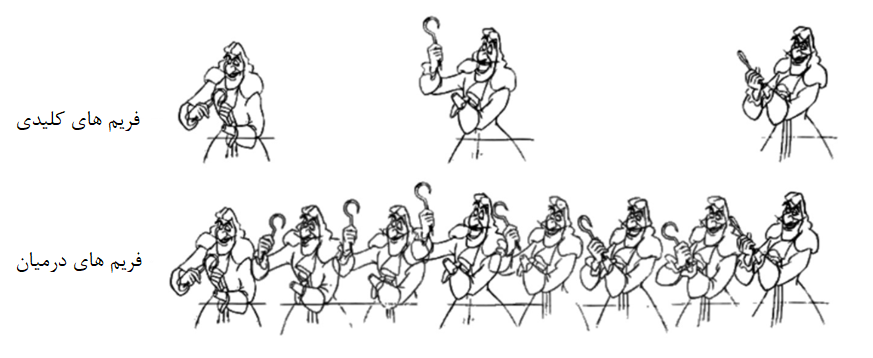
\includegraphics[width=\textwidth,height=\textheight,keepaspectratio]{Figures/Ch1/KeyframeAnimation.png}}

	\caption{فریم‌های کلیدی و درمیان}
	\label{fig:KeyframeAnimation}
\end{figure}

\subsection{چشم‌انداز چندمنظوره}

استفاده از چشم‌انداز چندمنظوره روش دیگری بود که در پویانمایی سنتی استفاده می‌شد.
هماطور که از تصویر زیر مشخص است، برای نمایش یک محیط از یک چشم‌انداز استفاده می‌شد.
این چشم‌انداز می‌توانست نشان دهنده‌ی محیط در فواصل مختلف باشد. در این صورت، زمانی که 
دوربین در صحنه حرکت می‌کرد این توهم را در مخاطب ایجاد می‌کرد که گویی در محیط در حال حرکت هستیم.

\begin{figure}[ht]
	\centerline{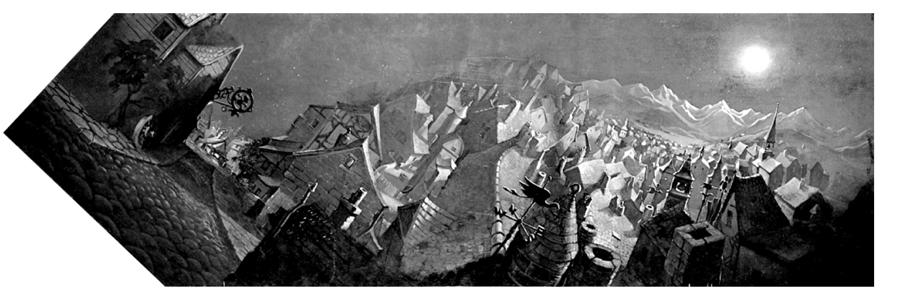
\includegraphics[width=\textwidth,height=\textheight,keepaspectratio]{Figures/Ch1/Panorama.png}}

	\caption{چشم‌انداز چندمنظوره}
	\label{fig:Panorama}
\end{figure}


\subsection{لایه‌های مختلف}

با استفاده از این روش، پویانما‌ها یک صحنه را به چند قسمت مختلف تقسیم می‌کردند.
به صورت مثال لایه‌های مختلف برای هر شخصیت درون صحنه استفاده می‌شد. علاوه برا ین یک لایه نیز برای تصویر پس‌زمینه استفاده می‌شد.
از آنجایی که این لایه‌ها یک صفحه‌ی شفاف بودند بنابراین می‌توان لایه‌‌ها را 
بر روی هم انباشته کرد و با تصویر برداری از بالا تمام صحنه را تصویربرداری کرد.
این روش در تصویر 
\ref{fig:DifferentLayers}
آورده شده است.

\begin{figure}[ht]
	\centerline{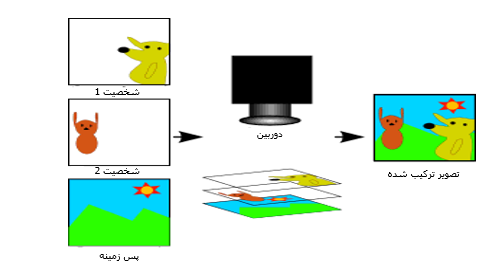
\includegraphics[width=\textwidth,height=\textheight,keepaspectratio]{Figures/Ch1/DifferentLayers.png}}

	\caption{لایه‌های مختلف}
	\label{fig:DifferentLayers}
\end{figure}

\section{پویانمایی کامپیوتری}

اگر بخواهیم نگاهی به تاریخچه‌ی انیمیشن‌های کامپیوتری بیاندازیم، مشاهده می‌کنیم که 
در حدود دهه‌ی 1980 میلادی شرکت دیزنی به عنوان یکی از اولین شرکت‌های جهان، شروع به 
دیجیتالی کردن خط لوله‌ی تولید پویانمایی سنتی خود کرد.
در این دیجیتال‌سازی بسیاری از روش‌ها و ایده‌‌های استفاده شده در پویانمایی سنتی،
به‌کار گرفته‌شد.
اولین مقالات این حوزه توسط آقای جان لستر از کارمندان پیکسار به عنوان 
"اصول پویانمایی سنتی به‌کار رفته در پویانمایی کامپیوتری سه‌بعدی"
ارائه شد.
در این مقاله اصول اولیه پویانمایی سنتی دوبعدی ترسیم شده با دست
و کاربرد آن‌ها در پویانمایی کامپیوتری سه‌بعدی شرح داده شده است.

پویانمایی کامپیوتری تنها محدود به دنیای سینما و فیلم‌های پویانمایی نمی‌شوند و به دنیای
بازی‌های کامپیوتری نیز ورود پیدا کرده‌اند. بازی‌های کامپیوتری سعی می‌کنند دیوار میان تماشاگران و فیلم را بشکنند و 
با تعاملی بودن و دادن آزادی عمل به بازیکن، سعی می‌کنند داستان را به گونه‌ای تعریف کنند که گویی بازیکن یکی از شخصیت‌های اصلی داستان است.
پویانمایی در بازی‌های کامپیوتری اهمیت بسیار بالایی دارد زیرا همانطور که گفته شد باعث 
جان بخشیدن به شخصیت‌ها می‌شود که اهمیت بسیار بالایی برای جلب توجه بازیکنان در هنگام داستان‌سرایی دارد.

با پیشرفت تکنولوژی، همراه با استفاده از روش‌های گذشته، روش‌های جدیدتری برای تولید پویانمایی توسعه یافته‌است که 
در ادامه به چند مورد از آن‌‌ها می‌پردازیم.

\subsection{فریم‌های کلیدی و درمیان}

همانطور که اشاره شد در پویانمایی کامپیوتری از روش‌های موجود در 
پویانمایی سنتی استفاده شده است. در اینجا نیز فریم‌های کلیدی 
یک حرکت توسط پویانماها به وجود می‌‌آیند ولی فریم‌های میانی به جای اینکه توسط پویانماها به وجود آید،
توسط کامپیوتر با استفاده از روش های درون‌یابی به وجود می‌آیند.

\subsection{رویه}

در این روش، حرکت بر اساس یک الگوریتم بیان می‌شود.
درواقع انیمیشن‌ها در این نوع پویانمایی، توابعی با تعداد کمی از متغیر‌ها هستند.
به عنوان مثال یک تابعی را درنظر بگیرید که به گرفتن ورودی ثانیه، دقیقه و ساعت، 
یک شئ ساعت را خروجی دهد که عقربه‌هایش در جای مناسب با توجه به ورودی‌ها قرار گرفته باشد.
حال می‌توان با تغییر ورودی‌ها حرکت ساعت را شبیه‌سازی کنیم.

\subsection{مبتنی بر فیزیک}

پویانمایی مبتنی بر فیزیک پلی میان دنیای پویانمایی با 
دنیای واقعی است. در این روش با نسبت دادن ویژگی‌های فیزیک به اشیاء سه‌بعدی و سپس حل‌کردن
فرمول‌های فیزیک مانند فرمول حرکت یا فرمول‌های نیوتن،
فیزیک را شبیه سازی می‌کند.
پویانمایی‌های مبتنی بر فیزیک شخصیت را قادر می‌سازد تا حرکت‌های خود را 
به صورت پویا با محیط تنظیم کند.

\subsection{ضبط حرکت
\protect \LTRfootnote{Motion Capture}}

به فرآیند ثبت و دیجیتالی‌کردن حرکت یک شئ یا شخص، ضبط حرکت گویند.
ضبط حرکت توسط دوربین‌های مادون قرمز که تعدادی زیادی از آن‌ها در صحنه‌ی ضبط قرار دارند، صورت می‌گیرد.
این دوربین‌ها به صورت شبکه به یکدیگر متصل هستند و پس از کالیبره شدن، آماده‌ی استفاده هستند.
این دوربین‌ها با استفاده از نشانگر‌های سفیدی که بر روی لباس بازیگران 
ضبط حرکت قرار دارد، داده‌های مورد نیازشان را دریافت می‌کنند.
قابل ذکر است این نشانگر‌ها بازتابنده‌ی مادون قرمز هستند.
در نهایت پویانماها به پاکسازی و پردازش این داده‌ها پرداخته تا آن را 
برای استفاده‌ی شخصیت‌های سه بعدی آماده کنند.



\section{موتور بازی‌سازی}
موتور‌های بازی‌سازی پلتفرم‌هایی هستند که ساخت بازی‌های رایانه‌ای را آسان‌تر می‌کنند.
آن ها به شما این امکان را می‌دهند تا عناصر بازی مانند انیمیشن، تعامل با کاربر یا تشخیص برخورد میان اشیاء را در یک واحد ادغام و ترکیب کنید.
\cite{barczak2019comparative}
زمانی که از اصطلاح موتور بازی‌سازی استفاده می‌کنیم منظورمان نرم‌افزارهای قابل توسعه‌ای هستند که می توانند پایه و اساس بسیاری از بازی‌های مختلف باشند.
\cite{GameEngineArchitecture}
موتورهای بازی‌سازی متشکل از اجزای مختلفی هستند که قابلیت‌های لازم برای ساخت بازی را فراهم می‌کنند.
رایج ترین اجزای موتور بازی عبارتند از:
\cite{barczak2019comparative}
\begin{itemize}
    \item[-] مولفه‌ی صدا: نقش اصلی این مولفه تولید جلوه‌های صوتی در بازی است.
    \item[-] موتور رندر: وظیفه اصلی این مولفه تبدیل داده‌های ورودی به پیکسل‌ها، برای به تصویر کشاندن بر روی صفحه است.
    \item[-] مولفه هوش مصنوعی: این مولفه مسئولیت ارائه‌ی تکنیک‌هایی برای تعریف قوانین رفتار شخصیت‌هایی را دارد که توسط بازیکنان کنترل نمی‌شوند.
    \item[-] مولفه انیمیشن: نقش اصلی این مولفه اجرای انیمیشن‌های مختلف مانند حرکت است.
    \item[-] مولفه شبکه: وظیفه اصلی این مولفه قادرساختنِ بازیِ همزمانِ بازیکنان با یکدیگر، از طریق استفاده از دستگاه‌های متصل به اینترنت است.
    \item[-] مولفه منطق یا مکانیک بازی: این مولفه قوانین حاکم بر دنیای مجازی، ویژگی‌های شخصیت‌های بازیکنان، هوش مصنوعی و اشیاء موجود در دنیای مجازی و همچنین وظایف و اهداف بازیکنان را تعریف می‌کند.
    \item[-] ابزارهای نرم‌افزاری: وظیفه اصلی این ابزارها افزایش راندمان و سرعت تولید بازی با موتور بازی‌سازی است. آن‌ها توانایی اضافه‌کردن بسیاری از عناصر مختلف را به بازی‌ها، از انیمیشن و جلوه‌های صوتی گرفته تا الگوریتم‌های هوش مصنوعی، را فراهم می‌کنند.   
\end{itemize}

یکی از مهم‌ترین مولفه‌های موجود در هر موتور بازی، مولفه‌ی انیمیشن آن است. در این پروژه به بررسی سیستم
انیمیشن گراف که وظیفه‌ی پخش انیمیشن‌ شخصیت‌های سه‌بعدی را در موتور بازی آنریل دارد می‌پردازیم.



\section {موتور بازی‌سازی آنریل}

اولین نسل موتور بازی‌سازی آنریل توسط تیم سوینی، بنیانگذار اپیک گیمز
\LTRfootnote {Epic Games}
،
توسعه یافت.
سویینی در سال 1995 شروع به نوشتن این موتور برای تولید بازی‌ تیراندازی اول شخصی به اسم غیرواقعی
\LTRfootnote{Unreal}
کرد.


نسخه‌‌ی دوم موتور بازی‌سازی آنریل در سال 2002 منتشر شد. 

نسخه سوم نیز در سال 2004 پس از حدود 18 ماه توسعه، منتشر شد.
در این نسخه، معماری پایه‌ای موجود در نسخه‌ی اول مانند طراحی شی‌گرا، اسکریپت‌نویسی مبتنی بر داده و رویکرد نسبتا ماژولار نسبت به زیرسیستم‌ها وجود داشت.
اما برخلاف نسخه دوم که از یک خط لوله با عملکرد ثابت
\LTRfootnote{fixed-function pipeline}
استفاده می‌کرد، این نسخه به صورتی طراحی شده بود تا بتوان قسمت‌های سایه‌زنی سخت‌افزاری
\LTRfootnote{shader hardware}
را برنامه‌نویسی کرد.


موتور بازی‌سازی آنریل 4 در سال 2014 در کنفرانس توسعه‌دهندگان بازی
\LTRfootnote{GDC}
منتشر شد.
این نسخه با طرح کسب‌و‌کار اشتراکی برای توسعه‌دهندگان در دسترس قرار گرفت. این اشتراک به صورت ماهانه، با پرداخت 19 دلار آمریکا به توسعه‌دهندگان این اجازه را می‌داد تا به نسخه‌ی کامل موتور، از جمله کد منبع 
\lr {C++}
آن
دسترسی پیدا‌ کنند.
البته در سال 2015 اپیک گیمز موتور بازی‌سازی آنریل را به صورت رایگان برای همگان منتشر ساخت.

آخرین نسخه آنریل به اسم موتور بازی‌سازی آنریل 5 در سال 2020 معرفی شد. این نسخه از تمام سیستم‌های موجود از جمله کنسول‌های نسل بعدی پلی‌استیشن 5
\LTRfootnote{PlayStation 5}
و ایکس‌باکس سری 
\lr{X/S}
\LTRfootnote{Xbox Series X/S}
پشتیبانی می کند.
کار بر روی این موتور حدود دو سال قبل از معرفی آن شروع شده بود. در سال 2021 نسخه‌ای از آن به صورت دسترسی اولیه منتشر شد. به طور رسمی در سال 2022 نسخه‌ی کامل این موتور برای توسعه‌دهندگان انتشار یافت.
\cite{UnrealEngineWikiPedia}

\chapter {آشنایی با موتور بازی}

\section{ساخت پروژه}

برای اینکه بتوان از موتور بازی‌سازی آنریل استفاده کرد ، ابتدا باید پروژه ای متناسب با کاری که می‌خواهیم انجام دهیم، بسازیم.
\\
برای ساختن پروژه به صورت زیر عمل می‌کنیم.
\\
ابتدا مرورگر آنریل انجین را باز می‌کنیم.


سپس با انتخاب دسته بندی مناسب و انتخاب گزینه‌ی بعدی به صفحه‌ی زیر هدایت می‌شویم. در اینجا  زیرمجموعه‌ی بازی را انتخاب شده است.

\begin{figure}[H]
	\centerline{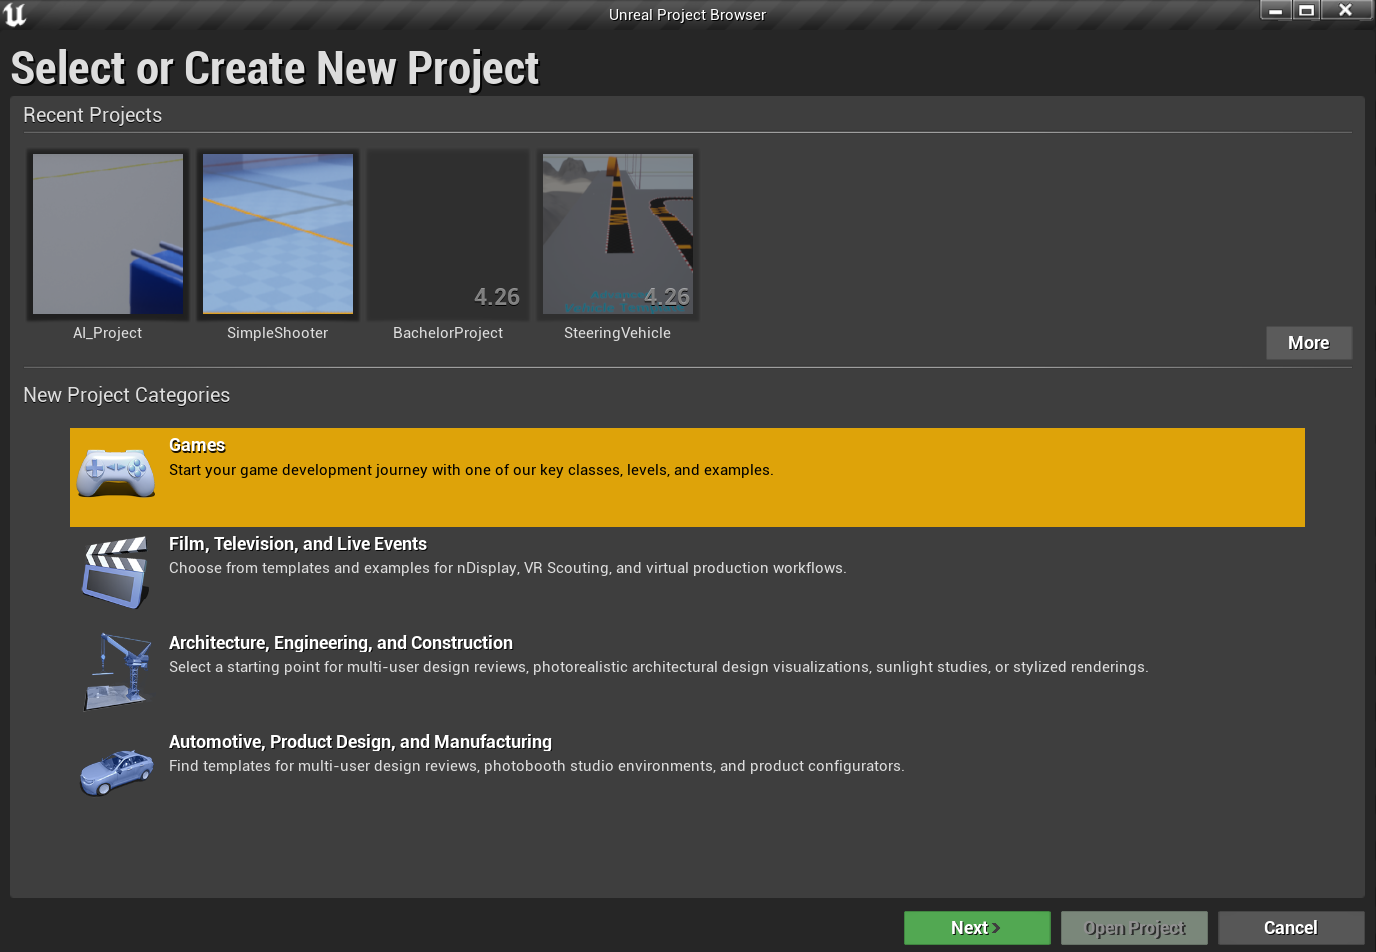
\includegraphics[width=\textwidth,height=\textheight,keepaspectratio]{Figures/Ch2/UnrealEngineBrowser.png}}
	\caption{مرورگر پروژه‌های آنریل}
	\label{fig:Unreal engine Browser}
\end{figure}

\par\bigskip 
\noindent


در اینجا قالب مناسب را انتخاب کرده و گزینه‌ی بعدی را کلیک می‌کنیم.

\begin{figure}[H]
	%\centerline{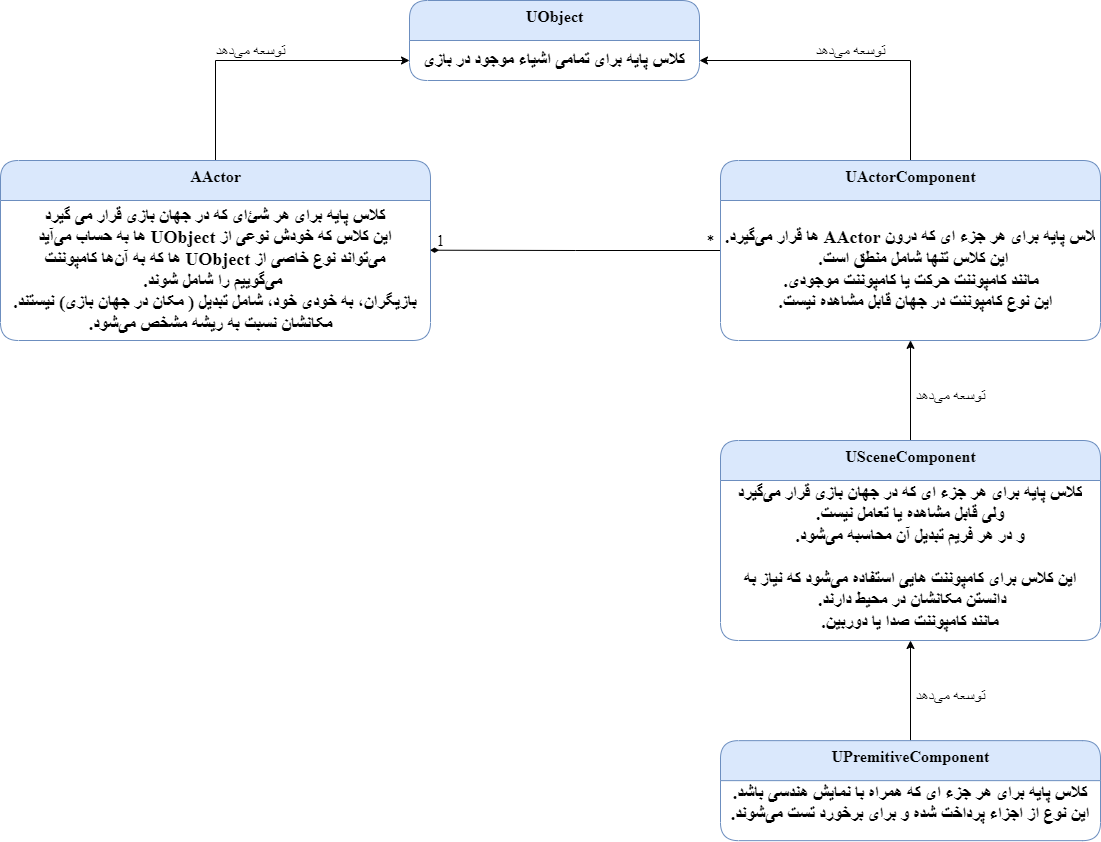
\includegraphics[scale=0.5]{Figures/Ch2/UnrealEngineBasicClassesUML.png}}
	\centerline{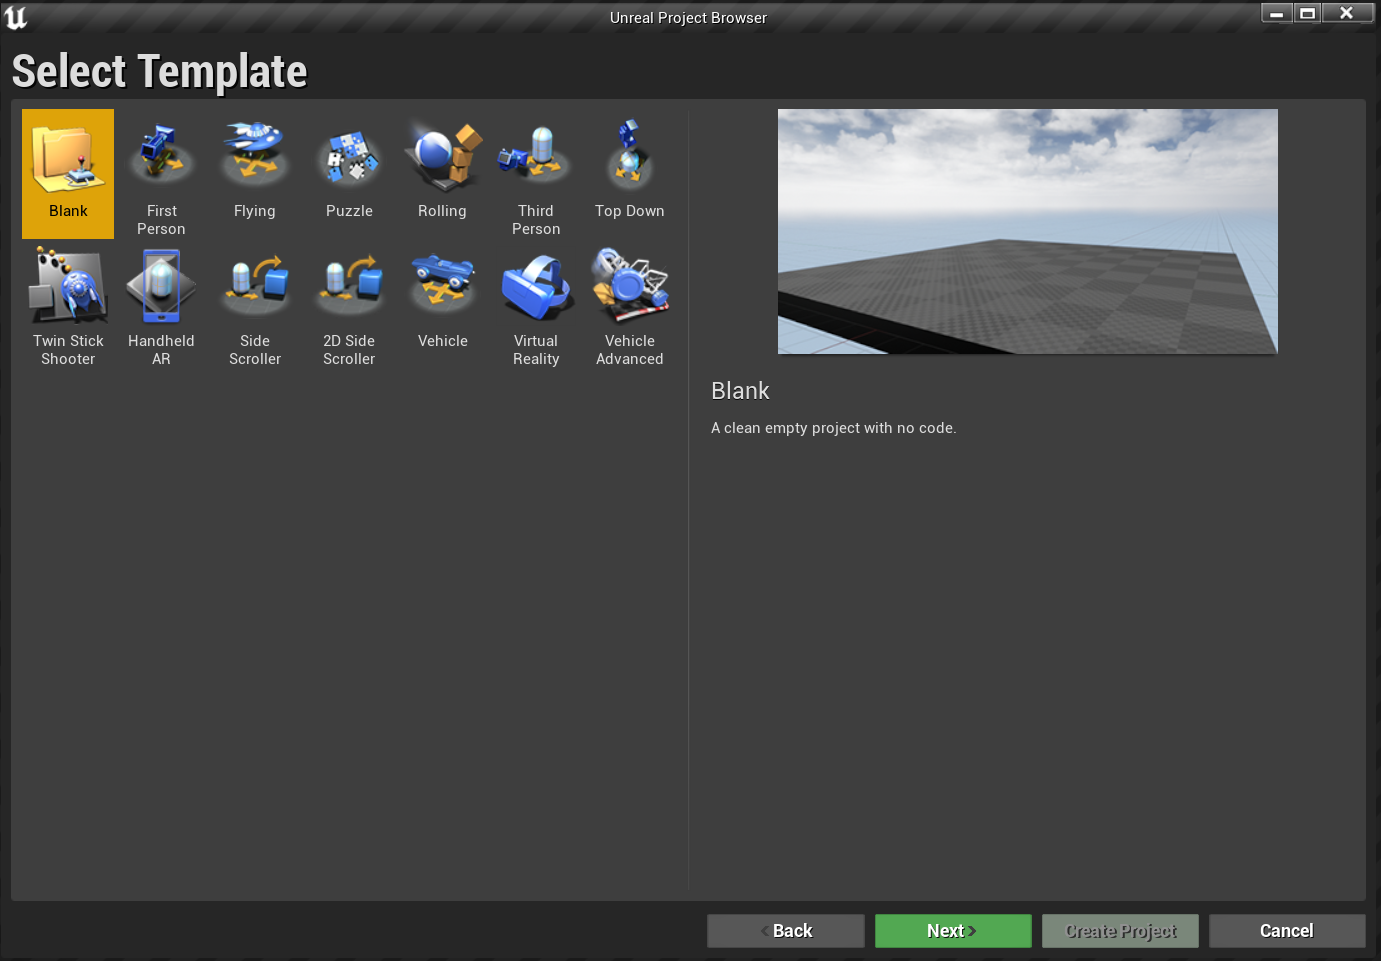
\includegraphics[width=\textwidth,height=\textheight,keepaspectratio]{Figures/Ch2/TemplateSelection.png}}

	\caption{قالب پروژه‌های آنریل}
	\label{fig:Unreal engine Template}
  \end{figure}





در اینجا پس از انجام تنظیمات اولیه پروژه گزینه‌ی ایجاد پروژه را کلیک کرده و پروژه ساخته می‌شود.


\begin{figure}[H]
	\centerline{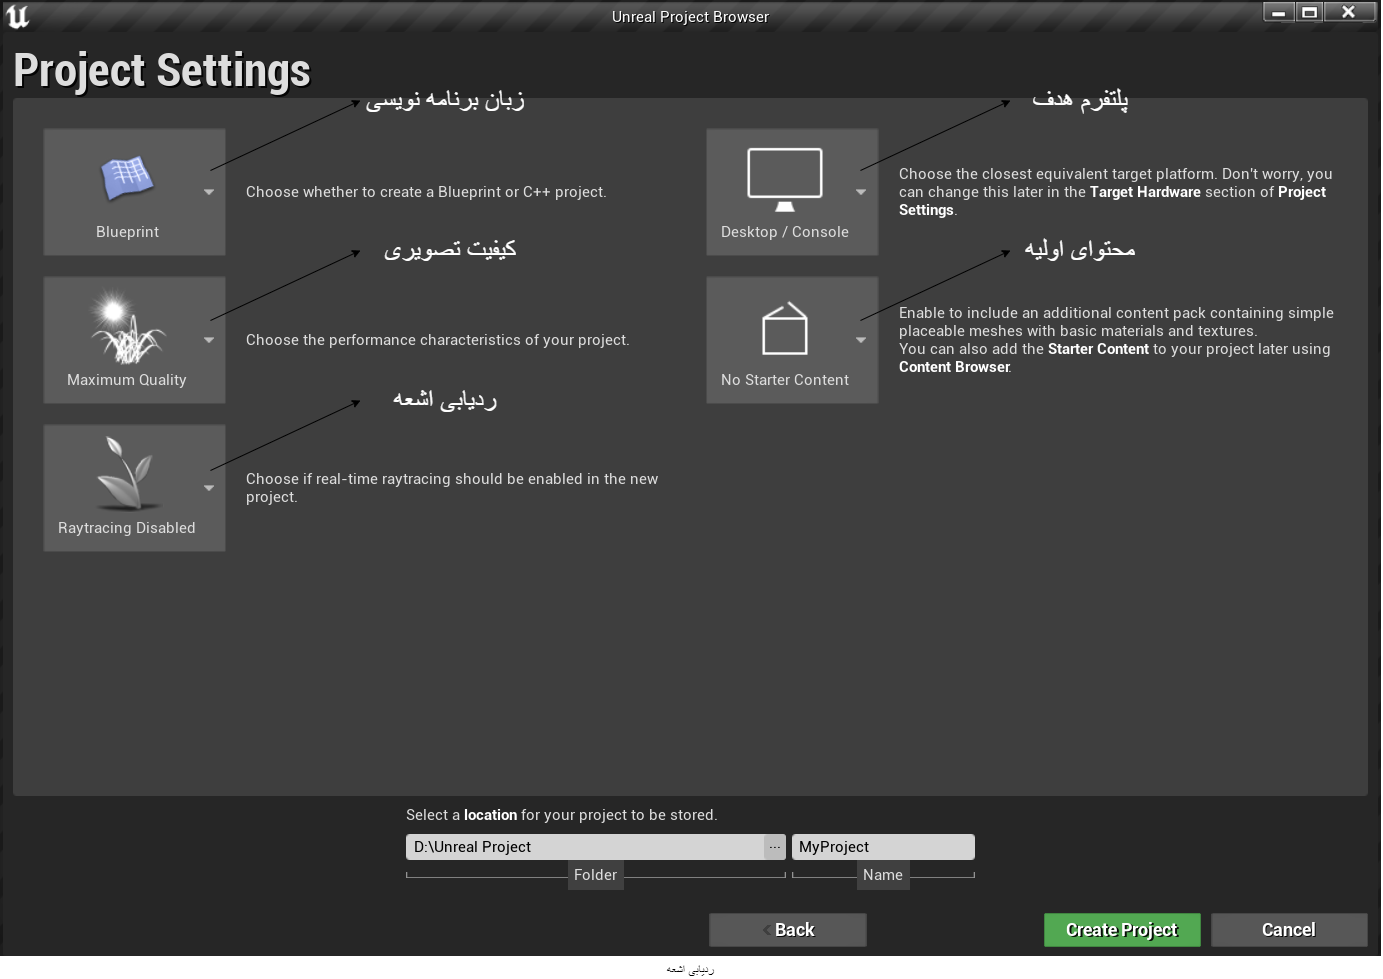
\includegraphics[width=\textwidth,height=\textheight,keepaspectratio]{Figures/Ch2/UnrealEngineProjectSetting.png}}
	\caption{تنظیم پروژه‌های آنریل}
	\label{fig:Unreal engine Setting}
\end{figure}


\section{ویرایشگر آنریل}
زمانی که پروژه ساخته می‌‌شود، ویرایشگر آنریل باز می‌شود. این ویرایشگر شامل پنل های مختلفی است که در عکس شماره زده شده و هر شماره نیز در جدول زیر توضیح داده شده است.

\begin{figure}[H]
	\centerline{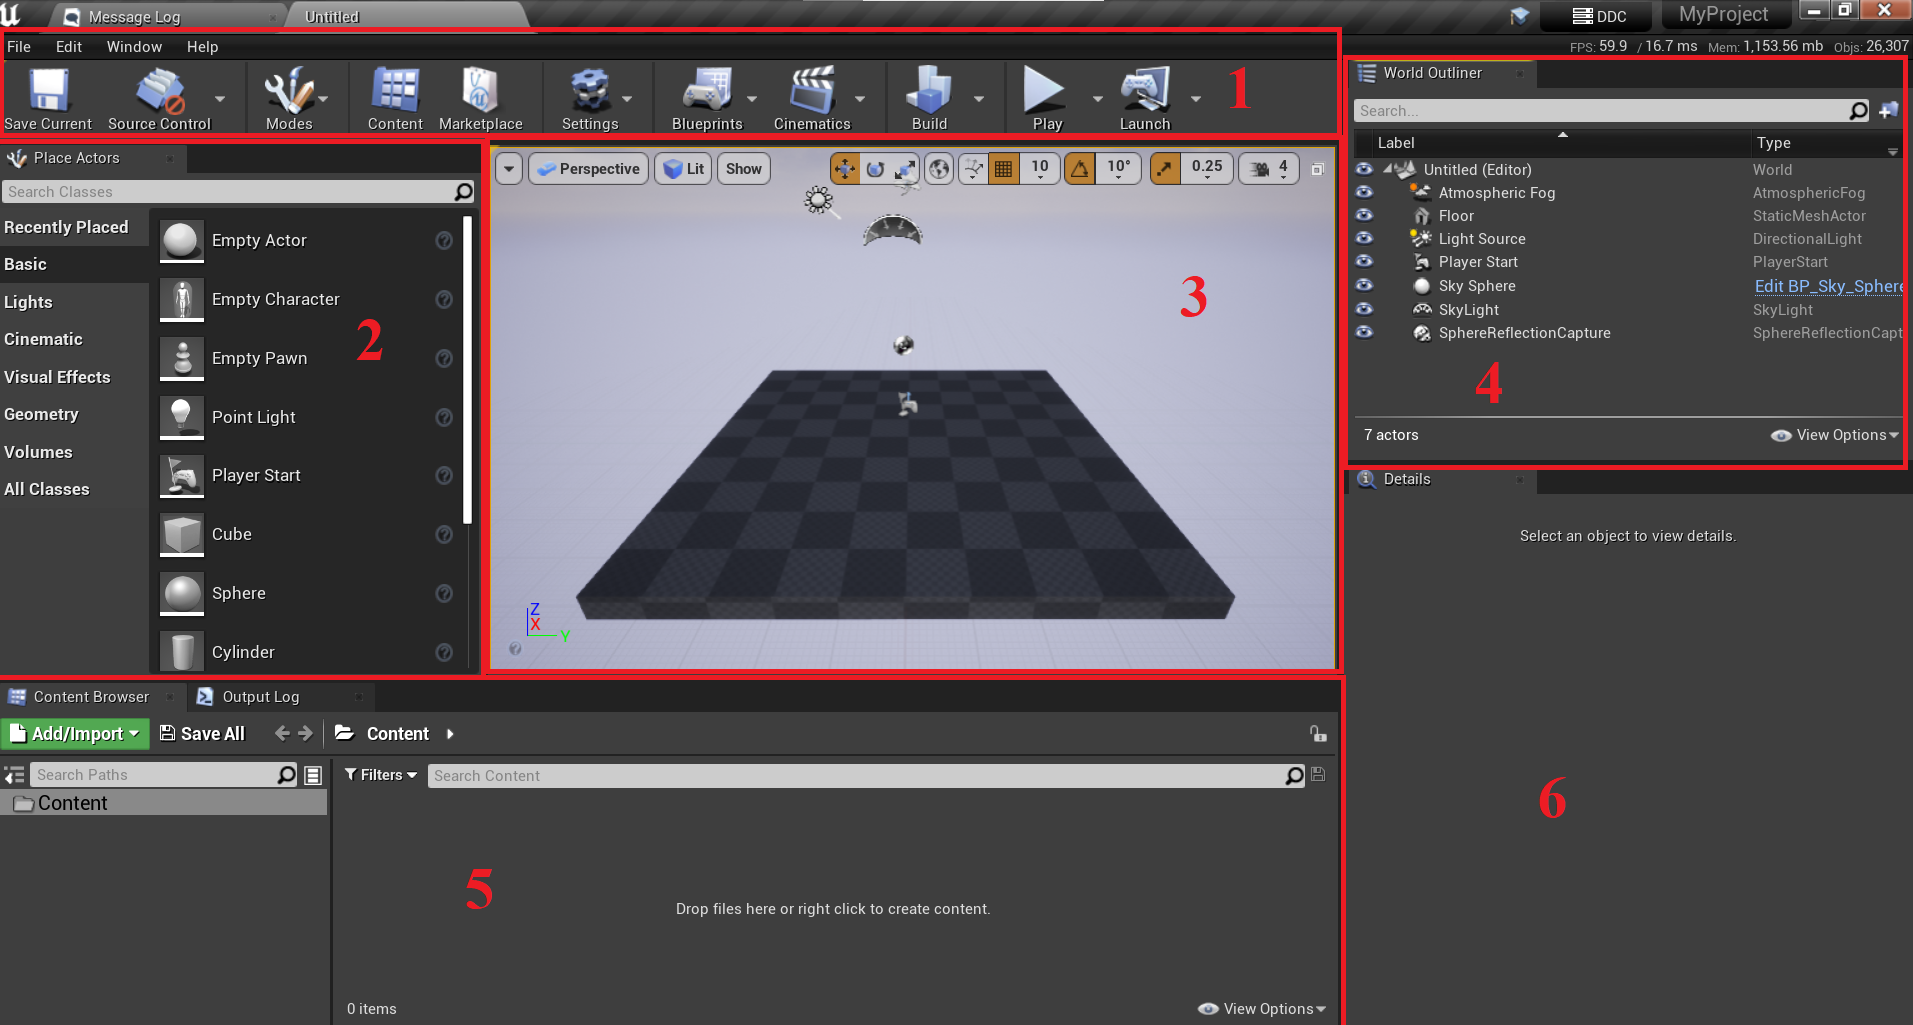
\includegraphics[width=\textwidth,height=\textheight,keepaspectratio]{Figures/Ch2/UnrealEngineEditor.png}}
	\caption{ویرایشگر آنریل}
	\label{fig:Unreal engine Editor}
\end{figure}

\begin{table}[ht]
	\caption{مدلهای تبدیل.}
	\label{tab:MotionModels}
	\centering
	\onehalfspacing
	\resizebox{\textwidth}{!}{
	\begin{tabular}{|r|c|l|r|}
		\hline شماره & نام &  \makecell{توضیح} \\ 
		\hline 1 & نوار ابزار & \makecell{شامل توابع مختلفی است که به صورت معمول استفاده می‌شود}\\ 
		\hline 2 & بازیگران &   \makecell{می‌توان از این قسمت، بازیگر مناسب خود را انتخاب کرده و در صحنه‌ی بازی قرار داد}\\ 
		\hline 3 & درگاه دید
		\LTRfootnote{Viewport} & \makecell{از طریق این پنل می‌توان اشیاء را در محیط قرار داد و بر روی اشیاء قرار گرفته شده کلیک کرد.}  \\ 
		\hline 4 & طرح کلی جهان
		\LTRfootnote{World Outliner} &  \makecell{تمامی اشیاء در مرحله فعلی را نشان می‌دهد. \\
		 می‌توان اشیا را با قرار دادن آن‌ها در پوشا‌ها سازماندهی کرد. همچنین قابلیت جستجو بر اساس نوع را نیز دارد.}\\
		\hline 5 & مرورگر محتوا & \makecell{این پنل تمامی فایل‌های پروژه را نمایش می‌دهد. \\ همچنین می‌توان با ایجاد پوشه فایل‌ها را دسته بندی و مرتب کرد. \\ علاوه بر این با استفاده از نوار جستجو می‌توان فایل موردنظر خود را پیدا کرد}\\ 
		\hline 6 & جزئیات & \makecell{ این پنل برای نمایش یا تغییر ویژگی‌های شئ انتخاب شده است.\\
		 با تغییر ویژگی‌ها تنها ویژگی شی انتخاب شده تغییر پیدا می‌کند.} \\ 
		\hline 
	\end{tabular} }
\end{table}

\section{زبان برنامه‌نویسی}

موتور بازی‌سازی آنریل از زبان برنامه نویسی 
\lr{C++}
به همراه اسکریپ بصری به نام 
\lr{Blueprint}
استفاده می‌کند.

\lr{Blueprint}
یک سیستم برنامه‌نویسی کامل گیمپلی مبتنی بر مفهوم استفاده از رابط‌های مبتنی بر گره برای ایجاد عناصر گیمپلی از درون ویرایشگر است.
این سیستم بسیار منعطف و قدرتمند است زیرا این توانایی را در اختیار طراحان قرار می دهد تا از طیف گسترده ای از مفاهیم و ابزارها که عموماً فقط در دسترس برنامه نویسان هستند استفاده کنند.
\cite{UnrealEngineBlueprint}

\section{رایج‌ترین اصطلاحات}

در این بخش رایج‌ترین اصطلاحات مورد استفاده در هنگام کار با موتور بازی‌سازی آنریل را بررسی می‌کنیم.

\subsection{ پروژه }

یک پروژه آنریل، شامل تمامی محتوای بازی است. 
محتوا می تواند خود به چندین پوشه که بر روی دیسک قرار دارند، تقسیم شود.
بدیهی است که می توان این پوشه‌ها را به صورت دلخواه نامگذاری و سازماندهی کرد.
پنل مروگر محتوا داخل ویرایشگر آنریل همان ساختار راهنمای موجود در پوشه 
\lr{Project}
که بر روی دیسک قرار دارد را نشان می‌دهد.

هر پروژه دارای یک پرونده‌‌ی
\lr{.uproject}
متناظر به خود است.این فایل نحوه ایجاد، باز کردن یا ذخیره یک پروژه است. بنابراین می‌توان چندین پروژه مختلف ایجاد کرد و به صورت موازی بر روی آن‌ها کار کرد.

\subsection{
شئ
}

اشیاء پایه‌ای ترین کلاس موجود در آنریل هستند. آنها مانند بلوک‌های سازنده عمل می‌کنند و دارای بسیاری از عملکرد‌ها و توابع موردنیاز برای دارایی‌ها
\lr{Assets}
هستند.


\subsection{
بازیگران \protect\LTRfootnote{Actors}
}

هر شئ‌ای را که بتوان بر روی صحنه قرار داد مانند دوربین، مش استاتیک، محل شروع بازی و ... را بازیگر
\LTRfootnote{Actor}
می‌گویند.
بازیگران از تبدیل‌های سه‌بعدی مانند انتقال، دوران و تغییر مقیاس پشتیبانی می‌کنند.
آن‌ها را می‌توان از طریق کد‌های گیمپلی (
	\lr{C++}
	یا برنامه‌کار 
	\LTRfootnote{Blueprint}
)
ایجاد کرد و یا از بین برد.

\subsection{تغییر نوع داده 
\protect\LTRfootnote{Casting}}

تغییر نوع داده، عملی است که طی آن بازیگری از یک کلاس را گرفته و سعی می‌کند به گونه‌ای رفتار کند که گویی از کلاس دیگری است.
این عمل ممکن است موفقیت آمیز باشد و یا شکست بخورد. در صورت موفقیت آمیز بودن می‌توان به توابع کلاسی که به آن تغییر داده شده دستیابی پیدا کرد.


\chapter { انیمیشن‌های اسکلتونی }

%{
%در این فصل برای پیا‌ده‌سازی سیستم انیمیشن به دنبال ارضا کردن 4 هدف کلی هستیم.
%\begin{enumerate}
%	\item نمایش اسکلت شخصیت در یک محیط سه‌بعدی
%	\item نمایش انیمیشن‌های سه‌بعدی اسکلت
%	\item نمایش شخصیت دارای مدل و اجرای انیمیشن بر روی آن
% 	\item با پیاده‌سازی روش ترکیب برای ترکیب انیمیشن‌های مختلف با یکدیگر
%\end{enumerate}

انیمیشن‌ اسکلتونی تکنیکی در انیمیشن‌های کامپیوتری است که به وسیله‌ی آن شخصیت‌های درون بازی متحرک می‌شوند. 
این سیستم به دو بخش کلی تقسیم می‌شود.
یک بخش،یک مش یا پوسته است که برای به نمایش کشاندن شخصیت در محیط سه‌بعدی استفاده می‌شود و بخش دوم یک اسکلت است. این اسکلت مجموعه سلسله مراتبی از قطعات به‌ هم پیوسته است که به هر قطعه یک مفصل گویند.
در این فصل به بررسی این دوبخش و تکنیک‌های موجود در انیمیشن‌های اسکلتونی خواهیم پرداخت

\section{مدل اسکلتونی}

در انیمیشن‌های اسکلتونی از مدل‌های اسکلتونی استفاده می‌شود. هر مدل اسکلتونی از دو بخش مدل و اسکلت تشکیل‌شده‌است. 

\section{شبکه‌ی\protect\LTRfootnote{Mesh} چندضلعی}

در گرافیک کامپیوتری سه‌بعدی و مدل‌سازی جامد، شبکه چند‌ضلعی مجموعه‌ای از رئوس، لبه‌ها و وجوه است که شکل یک جسم چند‌وجهی را مشخص می‌کند.
وجوه معمولاً از مثلث‌ها (شبکه مثلثی)، چهار ضلعی‌ها (چهار گوشه)، یا دیگر چند ضلعی‌های محدب ساده
(
	\lr{n}
	ضلعی‌ها
)
تشکیل شده‌اند. دلیل استفاده از این نوع چند ضلعی‌ها آسان‌تر بودن به نمایش‌کشیدن آن‌ها در محیط سه‌بعدی است.
البته در حالت کلی اشیاء ممکن است از چندضلعی‌های مقعر و یا حتی چندضلعی‌های دارای سوراخ نیز تشکیل‌شده‌باشند.

اشیاء ایجادشده توسط مش‌های چند ضلعی باید انواع مختلفی از عناصر، از جمله رئوس، لبه‌ها، وجوه، چندضلعی‌ها و سطوح را در خود ذخیره کنند.
در بسیاری از نرم‌افزارهای سه‌بعدی، فقط رئوس، لبه‌ها و یکی از دو مورد وجوه یا چند‌ضلعی‌ها ذخیره می‌شوند.
در اکثر سیستم‌های رندر
\LTRfootnote{renderer}
فقط از وجوه سه‌ضلعی
(مثلث‌ها)
استفاده‌ می‌شود.
بنابراین در این حالت چند‌ضلعی‌های مدل، باید به شکل مثلث باشند. البته سیستم‌های رندر‌ ای وجود دارند که از چهارضلعی‌ها یا چندضلعی‌های با تعداد اضلاع بالاتر نیز پشتیبانی ‌می‌کنند و یا در لحظه این چندضلعی‌ها را به مجموعه‌ای از مثلث‌ها تبدیل می‌کنند که در این صورت باعث ‌می‌شود نیازی به ذخیره‌ی مش به شکل مثلثی نباشد.

بنابراین چهار قسمت اصلی یک مش چندضلعی، رئوس، لبه‌ها، وجوه و چندضلعی‌ها هستند. توضیح کوتاهی درباره‌ی هر کدام از این موارد را در زیر می‌توانیم مشاهده کنیم.

\subsection{راس}
راس‌ها معمولا یک موقعیت در فضای سه‌بعدی همراه با اطلاعات دیگر مانند رنگ، بردار نرمال و مختصات بافت را شامل می‌شوند. 
در راس‌های مربوط به مش‌های اسکلتونی اطلاعاتی مانند تعداد مفاصلی که بر روی این راس تاثیر می‌گذارند همراه با وزن تاثیرگذاری آن‌ها، می‌تواند اضافه شود.

\subsection{لبه}
ارتباط بین دو راس را لبه گویند.

\subsection{وجه}
مجموعه‌ای بسته از لبه‌ها را وجه گویند. وجه‌ها می‌توانند از سه لبه 
(وجه مثلثی)
یا از چهار لبه
(وجه چهارگوش)
تشکیل شده باشند.

\subsection{چندضلعی}
یک چندضلعی مجموعه‌ای همسطح از وجوه است.
در سیستم‌هایی که از وجه‌های چند ضلعی پشتیبانی می‌کنند، وجوه و چندضلعی‌ها یکسان هستند ولی در صورتی که سیستم مورد نظر تنها از سه یا چهار ضلعی‌ها پشتیبانی کند، در این صورت به چند ضلعی‌ها، مجموعه‌ای از وجوه گفته می‌شود.

\section{مدل}

مدل‌
\footnote{ گاهی به جای استفاده از واژه‌ی مدل، از واژه‌ی مش هم استفاده می‌شود.}
درواقع هر شئ‌ای است که در محیط سه‌بعدی قرار می‌گیرد و به تصویر کشیده ‌می‌شود. هر مدل می‌تواند از چند زیرمش تشکیل شود.
به عنوان مثال یک ماشین را درنظر بگیریم. موجودیت ماشین می‌تواند یک مدل باشد که در محیط سه‌بعدی قرار می‌گیرد. مدل ماشین می‌تواند از چند زیرمش مانند چرخ‌ها، لاستیک‌ها و بدنه‌ی ماشین تشکیل شود. دلیل وجود داشتن یک موجودیت کلی به اسم ماشین این است که یک ‌شخصی مانند طراح محیط و یا طراح مرحله ‌نمی‌خواهد هر بار که ماشینی را در محیط قرار دهد، تک تک زیرمش‌ها را به صورت دستی در صحنه وارد کند و در سر جای خودش قرار بدهد.


\section{زیرمش
\protect\LTRfootnote{Sub-Mesh}
}
چندضلعی‌های دارای یک نوع ماده
\LTRfootnote{Material}
را یک زیرمش گویند.
همانطور که اشاره شد، هر مدل از چند زیرمش تشکیل می‌شود. دلیل این تقسیم این است که در هر عملیات به تصویر کشیدن
\LTRfootnote{Render}
تنها یک ماده می‌تواند به تصویر کشیده شود. مثلا در مثال ماشین، قسمت‌های مختلف ماشین از ماده‌های مختلفی تشکیل می‌شود. به طور مثال چرخ ماشین می‌تواند از جنس آلومینیوم باشد، لاستیک چرخ از جنس پلاستیک باشد و یا حتی قسمت‌های داخلی ماشین مانند صندلی ماشین، از جنس چرم باشد.
بنابراین باید این قسمت‌ها به صورت جدا قرار گیرند تا بتوان هر قسمت را با توجه به ماده‌ی موردنظر آن به تصویر کشاند.

\section{ماده 
\protect\LTRfootnote{Material}
}
ماده‌ها شامل پارامتر‌های قابل تنظیمی هستند که با تنظیم آن‌ها، به گرافیک اعلام می‌شود که چگونه باید یک مثلث را به تصویر بکشد.
این پارامترها می‌توانند شامل موارد زیر باشند ولی محدود به آن نمی‌شوند

\begin{enumerate}
	\item میزان کدورت و شفافیت شئ
 	\item میزان براقی شئ
 	\item رنگ(بافت) شئ
 	\item سایه‌زنی پیکسلی یا راسی \protect\LTRfootnote{Vertex or Pixel shader}
\end{enumerate}


\section{بافت
\protect\LTRfootnote{Texture}
}
بافت یک تصویر دوبعدی و یا سه‌بعدی است که می‌تواند در ماده استفاده شود.
این تصاویر به عنوان ورودی در برنامه دریافت شده و پس از اینکه یک شناسه به آن ها تخصیص داده شد، در کارت گرافیک قرار می‌گیرند. ماده‌ها با استفاده از این شناسه می‌توانند در صورت لزوم به این بافت‌ها دستیابی پیدا کنند.


\section{اسکلت}

به مجمو‌عه ای از مفاصل که به صورت سلسله مراتبی به یکدیگر متصل می‌شوند، اسکلت گویند. پس از آنکه هنرمندان مدل شخصیت را طراحی می‌کنند در طی یک مرحله که به آن
\lr{Rigging}
گویند، ساختار سلسله مراتبی اسکلت را به وجود می‌آورند.
در انیمیشن‌ها درواقع این اسکلت‌ است که حرکت می‌کند و با حرکتش باعث حرکت مدل شخصیت می‌شود.


\section{
\lr{Skinning}
}

تا اینجا با دو مفهوم مدل و اسکلت آشنایی پیدا کردیم ولی نگفتیم که این دو چگونه به هم مرتبط می‌شوند.
به عملیاتی که طی آن مفاصل موجود در اسکلت به مدل متصل می‌شود 
\lr{skinning}
گویند.
طی این مرحله هر راس موجود در پوسته‌ی مش به یک یا چند مفصل متصل می‌شود.
برای اینکه چگونه رئوس مش، این مفاصل را دنبال کنند الگوریتم‌های مختلفی مطرح شده‌است که در فصل پیاده‌سازی به یکی آن‌ها اشاره ‌خواهد شد.


\section{ژست شخصیت}

ژست یک شخصیت نشان‌دهنده‌ی نحوه‌ی قرارگیری مفصل‌ها در اسکلت است. ژست‌های مختلف با دروان، حرکت یا تغییر اندازه‌ی مفاصل درون اسکلت به وجود می‌‌آیند.
همانگونه که اشاره شد، اسکلت یک مدل در مرحله‌ی 
\lr{Rigging}
به وجود می‌‌آید و در همین مرحله با استفاده از 
\lr{ Skinning}
 به مدل متصل می‌شود. زمانی که این عمل صورت می‌گیرد مدل در یک ژست به خصوص قرار دارد که به آن ژست حالت اتصال
\LTRfootnote{Bind Pose}
یا
ژست مرجع
\LTRfootnote{Reference Pose}
گویند.
به صورت کلی شخصیت در این حالت به صورتی ایستاده‌است که پاهایش کمی از هم باز است و 
بازو‌هایش به شکل حرف
\lr{T}
کشیده است. به همین جهت گاهی به ژست حالت اتصال،
ژست
\lr{T}
\LTRfootnote{T Pose}
هم گفته می‌شود.
این حالت خاص به این دلیل انتخاب می‌شود که اندام‌ها را از بدن دور نگه دارد و اینکار باعث می‌شود که 
فرایند اتصال رئوس به مفصل آسان‌تر شود.

همانگونه که اشاره‌‌شد مفاصل به صورت سلسله مراتبی به یکدیگر متصل هستند. یعنی نحوه‌ی 
قرارگیری آن‌ها متناسب با نحوه‌ی قرارگیری والدشان است.
این کار باعث می‌شود که مفاصل به صورت طبیعی حرکت کنند. یعنی در صورتی که والد حرکت کند، به واسطه‌ی 
آن فرزند نیز حرکت می‌کند.
زمانی که ژست شخصیت در این حالت والد، فرزندی قرار دارد به آن ژست محلی
\LTRfootnote{Local Pose}
گفته می‌شود. حالت دیگری نیز وجود دارد که موقعیت هر مفصل نسبت به فضای مختصاتی مدل 
درنظر گرفته می‌شود. به ژست شخصیت در این حالت ژست جهانی
\LTRfootnote{Global Pose}
گفته می‌شود.

\section{‌کلیپ‌های انیمیشنی}

در یک فیلم انیمیشنی، تمام بخش‌های یک صحنه قبل از ساخت هر انیمیشن به دقت برنامه‌ریزی می‌شود.
این شامل حرکات هر شخصیت، لوازم موجود در صحنه و حتی حرکات دوربین نیز می‌شود.
این بدان معنی است که کل صحنه را می‌توان به عنوان یک دنباله طولانی و پیوسته از فریم‌ها، متحرک ساخت.
در این حالت در صورتی که شخصیتی خارج از دوربین هستند لازم نیستند که متحرک شوند.

کلیپ‌های انیمیشنی متفاوت از این هستند. یک بازی، یک تجربه‌ی تعاملی است بنابراین نمی‌توان از قبل چگونه حرکت کردن شخصیت‌ها و رفتار آن‌ها را پیش‌بینی کرد.
حتی تصمیمات شخصیت‌های غیربازیکن کامپیوتری نیز می‌توانند تابعی از اقدامات غیر قابل پیش‌بینی بازیکن انسانی باشد.
به این ترتیب، کلیپ‌های انیمیشنی مربوط به بازی تقریبا هیچ‌گاه از مجموعه‌ای از فریم‌های طولانی و به هم پیوسته تشکیل نمی‌شوند.
درعوض، حرکت شخصیت بازی باید به تعداد زیادی حرکات ریز تقسیم شود. 
منظور از کلیپ‌های انیمیشنی این حرکات کوتاه و یکتا است.

بنابراین هر کلیپ به صورتی طراحی شده است که یک عمل کاملا مشخص را انجام دهد. برخی از این کلیپ‌ها به گونه‌ای طراحی شده اند که بتوان آن را به صورت حلقه شونده تکرار کرد.
به عنوان مثال چرخه‌ی راه‌رفتن یا دویدن می‌توانند از این نوع کلیپ‌ها باشند.
و حرکاتی مانند پریدن یا دست تکان دادن از نوعی هستند که تنها یک‌بار پخش می‌شوند.

بنابراین به طور کلی حرکات هر شخصیت بازی معمولا به هزاران کلیپ تقسیم می‌شود. \cite{GameEngineArchitecture}

\section{ترکیب انیمیشن}

اصطلاح ترکیب انیمیشن به هر تکنیکی اطلاق می‌شود که در آن بیش از یک کلیپ انیمیشن در ژست نهایی کاراکتر سهیم می‌شود.
به صورت دقیق تر در این عمل دو یا چند ژست برای ایجاد یک ژست خروجی برای اسکلت شخصیت، با یکدیگر ترکیب می‌شوند.
همانطور که در بخش قبل گفته شد، کلیپ‌های انیمیشنی، کلیپ‌های کوتاه و یکتایی هستند. با استفاده از روش ترکیب ‌می‌توان مجموعه‌ای از کلیپ‌های انیمیشنی را با یکدیگر ترکیب کرد تا مجموعه‌ی جدیدی از انیمیشن‌ها را بدون نیاز به ایجاد دستی و از پایه‌ی آن ها تولید کنیم.
به عنوان مثال، با ترکیب یک انیمیشن راه رفتن آسیب دیده با راه رفتن بدون آسیب دیدگی، می‌توانیم سطوح مختلفی از آسیب دیدگی در هنگام راه‌رفتن را به وجود آوریم.
از ترکیب می‌توان برای درون‌یابی بین حالات مختلف چهره، حالت‌های مختلف بدن و حالت‌های مختلف حرکتی استفاده کرد.
از ترکیب می‌توان برای یافتن یا حالت میانی بین دو حالت شناخته شده در زمان‌های مختلف استفاده کرد. این‌کار زمانی استفاده می‌شود که بخواهیم ژست یک شخصیت را در نقطه‌ای از زمان پیدا کنیم که دقیقا با یکی از فریم‌های نمونه موجود در داده‌های انیمیشن مطابقت ندارد.
همچنین می‌توانیم از ترکیب موقتی انیمیشن برای انتقال هموار از یک انیمیشن به انیمیشن دیگر، با ترکیب تدریجی انیمیشن مبدا به مقصد در مدت زمان کوتاهی استفاده کنیم.
%\chapter {سیستم انیمیشن گراف در موتور بازی‌سازی آنریل}

در این فصل ابتدا توضیحاتی راجع به آنریل انجین داده می‌شود و سپس در رابطه‌ی سیستم انیمشن گراف این انجین صحبت خواهد شد.

\section{بازیگران، پیاده‌ها و شخصیت‌‌ها}

اشیا در آنریل می‌توانند به سه کلاس کلی بازیگران، پیاده‌ها و شخصیت‌ها دسته‌بندی می‌شوند.
بازیگران کلاس پایه‌ی تمامی اشیا ای هستند که به صورت فیزیکی می‌توانند در محیط سه‌بعدی قرار گیرند.
پیاده‌ها کلاسی مشتق شده از بازیگران هستند که بازیکنان می‌توانند کنترل آن‌ها را بدست گیرند و 
در محیط حرکت کنند.
 و در نهایت شخصیت‌ها پیاده‌هایی هستند که دارای مش اسکلتونی، توانایی شناسایی برخورد و منطق حرکتی هستند.
 آنها مسئول تمام تعاملات فیزیکی بین بازیکن یا هوش مصنوعی، با جهان هستند و همچنین مدل های اولیه شبکه و دریافت ورودی را پیاده سازی می کنند. 
اگر بخواهیم شخصیت درون بازی از انیمیشن‌های اسکلتونی استفاده کند، باید از این کلاس بهره ببریم.

\section{اجزاء}

اجزاء
\LTRfootnote{Components}
مجموعه‌ای از توابع و ویژگی‌ها است که می‌تواند به یک بازیگر اضافه شود.
بنابراین بازیگران می‌توانند حاوی مجموعه‌ای از
\lr{ActorComponents}
باشند که این اجزاء می‌توانند برای موارد مختلفی از جمله
کنترل نحوه‌ی حرکت بازیگران، 
نحوه‌ی رندر شدن و غیره استفاده شوند.

زمانی که یک مولفه به یک بازیگر اضافه می‌شود، آن بازیگر می‌تواند عملکرد‌های موجود در آن مولفه را استفاده کند.
به عنوان مثل یک مولفه نور نقطه‌ای باعث می‌شود که بازیگر مانند یک نور نقطه‌ای، نور ساطع کند.
یا یک مولفه صورتی به بازیگر این توانایی پخش صدا را می‌دهد.

مولفه‌ها حتما باید به یک بازیگر متصل شوند و به خودی خود نمی‌توانند وجود داشته باشند.
درواقع وقتی ما مولفه‌های مختلف را به بازیگر خود متصل می‌کنیم درواقع در حال قرار دادن قطعه‌ها و تکه‌هایی هستیم
 که مجموع آن‌ها یک بازیگر را به عنوان یک موجودیت واحد که در محیط سه‌بعدی قرار می‌گیرد تعریف می‌کنند.
 به عنوان مثال چرخ‌های یک ماشین، فرمان ماشین، چراغ‌ها و غیره همه به عنوان
 مولفه‌های ماشین درنظر گرفته می‌شوند در حالی که خود آن ماشین، بازیگر است.

\section{شخصیت‌ها}

هر شخصیت در آنریل از سه مولفه‌ی اصلی تشکیل شده است.


\begin{itemize}
	\item \lr{Skeletal Mesh Component}
	\item \lr{Character Movement Component}
	\item \lr{Capsule Component}
\end{itemize}


همانطور که در فصل‌های گذشته اشاره‌شد شخصیت‌ها برای پخش انیمیشن‌‌ها نیاز به یک مش اسکلتونی دارند.
مولفه‌ی 
\lr{Skeletal mesh Component }
 مش اسکلتونی اصلی مرتبط با شخصیت است.
این مولفه‌ای است که برای ما در این پروژه اهمیت زیادی دارد.

مولفه‌ی 
\lr{ Character Movement Component}
همانطور که از اسمش مشخص است برای منطق حرکت در حالت‌های مختلف از جمله راه‌رفتن افتادن و غیره استفاده می‌شود.
این مولفه شامل تنظیمات و عملکرد‌های مربوطه برای کنترل حرکت است.

و در نهایت مولفه‌‌ی
\lr{Capsule Component}
وظیفه‌ی تشخیص برخورد در هنگام حرکت را دارد.



%\chapter { انیمیشن‌های اسکلتونی }

%{
%در این فصل برای پیا‌ده‌سازی سیستم انیمیشن به دنبال ارضا کردن 4 هدف کلی هستیم.
%\begin{enumerate}
%	\item نمایش اسکلت شخصیت در یک محیط سه‌بعدی
%	\item نمایش انیمیشن‌های سه‌بعدی اسکلت
%	\item نمایش شخصیت دارای مدل و اجرای انیمیشن بر روی آن
% 	\item با پیاده‌سازی روش ترکیب برای ترکیب انیمیشن‌های مختلف با یکدیگر
%\end{enumerate}

انیمیشن‌ اسکلتونی تکنیکی در انیمیشن‌های کامپیوتری است که در آن شخصیت درون بازی به دوبخش تقسیم ‌می‌شود. یک بخش،یک مش یا پوسته است که برای به نمایش کشاندن ‌آن شخصیت در محیط سه‌بعدی استفاده می‌شود و بخش دوم یک اسکلت است. این اسکلت مجموعه سلسله مراتبی از قطعات به‌ هم پیوسته است که به هر قطعه یک مفصل گویند.
در این فصل به بررسی این دوبخش و تکنیک‌های موجود در انیمیشن‌های اسکلتونی خواهیم پرداخت

\section{مدل اسکلتونی}

در انیمیشن‌های اسکلتونی از مدل‌های اسکلتونی استفاده می‌شود. هر مدل اسکلتونی از دو بخش مدل و اسکلت تشکیل شده است. 

\section{شبکه‌ی\protect\LTRfootnote{Mesh} چندضلعی}

.در گرافیک کامپیوتری سه‌بعدی و مدل‌سازی جامد، شبکه چند‌ضلعی مجموعه‌ای از رئوس، لبه‌ها و وجوه است که شکل یک جسم چند‌وجهی را مشخص می‌کند
وجه‌ها معمولاً از مثلث‌ها (شبکه مثلثی)، چهار ضلعی (چهار گوشه)، یا دیگر چند ضلعی‌های محدب ساده
(
	\lr{n}
	ضلعی‌ها
)
تشکیل شده‌اند. دلیل استفاده از این نوع چند ضلعی‌ها آسان‌تر بودن به نمایش کشیدن وجوه در محیط سه‌بعدی است.
البته در حالت کلی اشیاء ممکن است از چندضلعی‌های مقعر و یا حتی چندضلعی‌های دارای سوراخ نیز تشکیل شده باشند.

اشیاء ایجادشده توسط مش‌های چند ضلعی باید انواع مختلفی از عناصر، از جمله رئوس، لبه‌ها، وجوه، چندضلعی‌ها و سطوح را ذخیره کنند.
در بسیاری از نرم‌افزارهای سه‌بعدی، فقط رئوس، لبه‌ها و یکی از دو مورد وجوه یا چند‌ضلعی‌ها ذخیره می‌شوند.
در اکثر سیستم‌های رندرکننده
\LTRfootnote{renderer}
فقط از وجوه سه‌ضلعی
(مثلث‌ها)
استفاده‌ می‌شود.
بنابراین در این حالت چند‌ضلعی‌های مدل باید به شکل مثلث باشند. البته سیستم‌های رندرای وجود دارند که از چهارضلعی‌ها یا چندضلعی‌های با تعداد اضلاع بالاتر نیز پشتیبانی ‌می‌کنند و یا در لحظه این چندضلعی‌ها را به مجموعه‌ای از مثلث‌ها تبدیل می‌کنند که در این صورت باعث ‌می‌شود نیازی به ذخیره‌ی مش به شکل مثلثی نباشد.

بنابراین چهار قسمت اصلی یک مش چندضلعی، رئوس، لبه‌ها، وجوه و چندضلعی‌ها هستند. توضیح کوتاهی درباره‌ی هر کدام از این موارد را در بخش زیر می‌توانیم مشاهده کنیم.

\subsection{راس}
راس‌ها معمولا یک موقعیت در فضای سه‌بعدی همراه با اطلاعات دیگر مانند رنگ، بردار نرمال، مختصات بافت 
در راس‌های مربوط به مش‌های اسکلتونی اطلاعاتی مانند تعداد مفاصلی که بر روی این راس تاثیر می‌گذارد همراه با وزن تاثیرگذاری‌اش می‌تواند اضافه شود.

\subsection{لبه}
ارتباط بین دو راس را لبه گویند.

\subsection{وجه}
مجموعه‌ای بسته از لبه‌ها را وجه گویند. وجه‌ها می‌توانند از سه لبه 
(وجه مثلثی)
یا از چهار لبه
(وجه چهارگوش)
تشکیل شده باشند.

\subsection{چندضلعی}
یک چندضلعی مجموعه‌ای همسطح از وجود است.
در سیستم‌هایی که از وجه‌های چند ضلعی پشتیبانی می‌کنند، وجوه و چندضلعی‌ها یکسان هستند ولی در صورتی که سیستم مورد نظر تنها از سه یا چهار ضلعی‌ها پشتیبانی کند، در این صورت چند ضلعی‌ها را مجموعه‌ای از وجوه گویند.

\section{مدل}

مدل‌
\footnote{ گاهی به جای استفاده از واژه‌ی مدل، از واژه‌ی مش هم استفاده می‌شود.}
درواقع هر شئ‌ای است که در محیط سه‌بعدی قرار می‌گیرد و به تصویر کشیده ‌می‌شود. هر مدل می‌تواند از چند زیرمش تشکیل شود.
به عنوان مثال یک ماشین را درنظر بگیریم. موجودیت ماشین می‌تواند یک مدل باشد که در محیط سه‌بعدی قرار می‌گیرد. مدل ماشین می‌تواند از چند زیرمش مانند چرخ‌ها، لاستیک‌ها و بدنه‌ی ماشین تشکیل شود. دلیل وجود داشتن یک موجودیت کلی به اسم ماشین این است که یک ‌شخصی مانند طراح محیط و یا طراح مرحله ‌نمی‌خواهد هر بار که ماشینی را در محیط قرار دهد، تک تک زیرمش‌ها را به صورت دستی در صحنه وارد کند و در سر جای خودش قرار بدهد.


\section{زیرمش
\protect\LTRfootnote{Sub-Mesh}
}
چندضلعی‌های دارای یک نوع ماده
\LTRfootnote{Material}
را یک زیرمش گویند.
همانطور که اشاره شد، هر مدل از چند زیرمش تشکیل می‌شود. دلیل این تقسیم این است که در هر عملیات به تصویر کشیدن
\LTRfootnote{Render}
تنها یک ماده می‌تواند به تصویر کشیده شود. مثلا در همان مثال ماشین، قسمت‌های مختلف ماشین از ماده‌های مختلفی تشکیل می‌شود. به طور مثال چرخ ماشین می‌تواند از جنس آلومینیوم باشد یا لاستیک چرخ از جنس پلاستیک باشد و یا حتی قسمت‌های داخلی ماشین مانند صندلی ماشین از جنس چرم باشد.
بنابراین باید این قسمت‌ها به صورت جدا قرار گیرند تا بتوان هر قسمت را با توجه به ماده‌ی موردنظر آن به تصویر کشاند.

\section{ماده 
\protect\LTRfootnote{Material}
}
ماده‌ها شامل پارامتر‌های قابل تنظیمی هستند که با تنظیم آن به گرافیک ما اعلام می‌کند که چگونه باید یک مثلث را به تصویر بکشد.
این پارامترها می‌توانند شامل موارد زیر باشند ولی محدود به آن نمی‌شوند

\begin{enumerate}
	\item میزان کدورت و شفافیت شئ
 	\item میزان براقی شئ
 	\item رنگ(بافت) شئ
 	\item سایه‌زنی پیکسلی یا راسی \protect\LTRfootnote{Vertex or Pixel shader}
\end{enumerate}


\section{بافت
\protect\LTRfootnote{Texture}
}
بافت یک تصویر دوبعدی و یا سه‌بعدی است که می‌تواند در ماده استفاده شود.
این تصاویر به عنوان ورودی در برنامه دریافت شده و پس از اینکه یک شناسه به آن ها تخصیص داده شد، در کارت گرافیکی قرار می‌گیرند. ماده‌ها با استفاده از این شناسه می‌توانند در صورت لزوم به این بافت دستیابی پیدا کنند.


\section{اسکلت}

به مجمو‌عه ای از مفاصل که به صورت سلسله مراتبی به یکدیگر متصل می‌شوند، اسکلت گویند. پس از آنکه هنرمندان مدل شخصیت را طراحی می‌کنند در طی یک مرحله که به آن
\lr{Rigging}
گویند، ساختار سلسله مراتبی اسکلت را به وجود می‌آورند.
در انیمیشن‌ها درواقع این اسکلت‌ است که حرکت می‌کند و با حرکتش باعث حرکت مدل شخصیت می‌شود.


\section{
\lr{Skinning}
}

تا اینجا با دو مفهوم مدل و اسکلت آشنایی پیدا کردیم ولی نگفتیم که این دو چگونه به هم مرتبط می‌شوند.
به عملیاتی که طی آن مفاصل موجود در اسکلت به مدل متصل می‌شود را 
\lr{skinning}
گویند.
طی این مرحله هر راس موجود در پوسته‌ی مش به یک یا چند مفصل متصل می‌شود.
برای اینکه چگونه رئوس مش، این مفاصل را دنبال کنند الگوریتم‌های مختلفی مطرح شده است که در فصل پیاده‌سازی به آن اشاره ‌خواهد شد.

\section{‌کلیپ‌های انیمیشنی}

در یک فیلم انیمیشنی، تمام بخش‌های یک صحنه قبل از ساخت هر انیمیشن به دقت برنامه‌ریزی می‌شود.
این شامل حرکات هر شخصیت، لوازم موجود در صحنه و حتی حرکات دوربین نیز می‌شود.
این بدان معنی است که کل صحنه را می‌توان به عنوان یک دنباله طولانی و پیوسته از فریم‌ها، متحرک ساخت.
در این حالت در صورتی که شخصیتی خارج از دوربین هستند لازم نیستند که متحرک شوند.

کلیپ‌های انیمیشنی متفاوت از این هستند. یک بازی، یک تجربه‌ی تعاملی است بنابراین نمی‌توان از قبل چگونه حرکت کردن شخصیت‌ها و رفتار آن‌ها را پیش‌بینی کرد.
حتی تصمیمات شخصیت‌های غیربازیکن کامپیوتری نیز می‌توانند تابعی از اقدامات غیر قابل پیش‌بینی بازیکن انسانی باشد.
به این ترتیب، کلیپ‌های انیمیشنی مربوط به بازی تقریبا هیچ‌گاه از مجموعه‌ای از فریم‌های طولانی و به هم پیوسته تشکیل نمی‌شوند.
درعوض، حرکت شخصیت بازی باید به تعداد زیادی حرکات ریز تقسیم شود. 
منظور از کلیپ‌های انیمیشنی این حرکات کوتاه و یکتا است.

بنابراین هر کلیپ به صورتی طراحی شده است که یک عمل کاملا مشخص را انجام دهد. برخی از این کلیپ‌ها به گونه‌ای طراحی شده اند که بتوان آن را به صورت حلقه شونده تکرار کرد.
به عنوان مثال چرخه‌ی راه‌رفتن یا دویدن می‌توانند از این نوع کلیپ‌ها باشند.
و حرکاتی مانند پریدن یا دست تکان دادن از نوعی هستند که تنها یک‌بار پخش می‌شوند.

بنابراین به طور کلی حرکات هر شخصیت بازی معمولا به هزاران کلیپ تقسیم می‌شود. \cite{GameEngineArchitecture}

\section{ترکیب انیمیشن}

اصطلاح ترکیب انیمیشن به هر تکنیکی اطلاق می‌شود که در آن بیش از یک کلیپ انیمیشن در ژست نهایی کاراکتر سهیم می‌شود.
به صورت دقیق تر در این عمل دو یا چند ژست برای ایجاد یک ژست خروجی برای اسکلت شخصیت، با یکدیگر ترکیب می‌شوند.
همانطور که در بخش قبل گفته شد، کلیپ‌های انیمیشنی، کلیپ‌های کوتاه و یکتایی هستند. با استفاده از روش ترکیب ‌می‌توان مجموعه‌ای از کلیپ‌های انیمیشنی را با یکدیگر ترکیب کرد تا مجموعه‌ی جدیدی از انیمیشن‌ها را بدون نیاز به ایجاد دستی و از پایه‌ی آن ها تولید کنیم.
به عنوان مثال، با ترکیب یک انیمیشن راه رفتن آسیب دیده با راه رفتن بدون آسیب دیدگی، می‌توانیم سطوح مختلفی از آسیب دیدگی در هنگام راه‌رفتن را به وجود آوریم.
از ترکیب می‌توان برای درون‌یابی بین حالات مختلف چهره، حالت‌های مختلف بدن و حالت‌های مختلف حرکتی استفاده کرد.
از ترکیب می‌توان برای یافتن یا حالت میانی بین دو حالت شناخته شده در زمان‌های مختلف استفاده کرد. این‌کار زمانی استفاده می‌شود که بخواهیم ژست یک شخصیت را در نقطه‌ای از زمان پیدا کنیم که دقیقا با یکی از فریم‌های نمونه موجود در داده‌های انیمیشن مطابقت ندارد.
همچنین می‌توانیم از ترکیب موقتی انیمیشن برای انتقال هموار از ک انیمیشن به انیمیشن دیگر، با ترکیب تدریجی انیمیشن مبدا به مقصد در مدت زمان کوتاهی استفاده کنیم.
\chapter { پیاده سازی }

در این بخش به روش‌ها و ابزارهای استفاده شده در پیاده‌سازی سیستم انیمیشن اشاره خواهد شد

\section {ابزارها}

\subsection {
    \lr{OpenGL}
    }

\lr{OpenGL}
یک واسط برنامه نویسی کاربردی  
\LTRfootnote{API}
است که با فراهم کردن توابع مختلف به توسعه‌دهندگان امکان دستکاری گرافیک و تصاویر را می‌دهد.
\lr{OpenGL} 
یک کتابخانه‌ی رندرینگ است.
یک "شئ" به خودی خود در
\lr{OpenGL} 
مفهومی ندارد
و به صورت مجموعه‌ای از مثلث‌ها و حالات مختلف درنظر گرفته می‌شود. بنابراین  
وظیفه‌ی ما است که بدانیم چه شئ‌ای در کدام قسمت صفحه رندر شده است. این کتابخانه تنها وظیفه‌اش، کشیدن تصاویری که است که می‌خواهیم به تصویر کشیده‌شوند.
در این صورت اگر می‌خواهیم تصویری را به‌روزرسانی کنیم و یا به عنوان مثال شئ‌ای را تحرک دهیم باید به 
\lr{OpenGL}
درخواست دهیم که صحنه را دوباره‌برای ما رندر کند.
\cite{KhronosUsingOpenGL}

به صورت کلی 
\lr{OpenGL}
را می‌توان یک ماشین حالت بزرگ درنظر گرفت. هر حالت شامل مجموعه‌ای از متغیر‌ها است که نحوه‌ی عملکرد
\lr{OpenGL}
را مشخص می‌کند. 
به مجموعه‌ی این حالت‌ها 
\lr{OpenGL context}
نیز می‌گویند. 
در واقع  
\lr{context}
را می‌توان یک شئ درنظر گرفت که کل
\lr{OpenGL}
را دربر می‌گیرد. عموما تمامی تغییرات، روی 
\lr{context}
فعلی اعمال می‌شود و سپس رندر می‌شود.
\cite{KhronosUsingOpenGL} \cite{LearnOpenGL_GettingStarted}

%%%%%%%%%%%%%%%%%%%%%%%%%%%%%%%%%%%%%%%%%%%%%%%%%%%%%

\subsection{\lr{GLFW}}

از آنجایی که به‌وجود‌آوردن یک پنجره‌ی جدید و همچنین 
\lr{context}
وابسته به نوع سیستم‌عامل است بنابراین نیازمند کتابخانه‌ای هستیم که بتواند این موارد را برای ما مدیریت کند.
\lr{GLFW}
یک کتابخانه‌ی منبع باز و چندپلتفرمی برای 
\lr{OpenGL}
است که یک
\lr{API}
ساده و مستقل از پلتفرم برای تولید پنجره‌ها، زمینه‌‌ها
\LTRfootnote{Contexts}
و سطوح، خواندن ورودی و مدیریت رویداد‌ها
\LTRfootnote{Events}
را ارائه می‌کند. 
این کتابخانه از سیستم‌عامل‌های 
ویندوز
، 
مک
و 
لینوکس
و سیستم‌های مشابه یونیکس پشتیبانی ‌می‌کند.
\cite{GLFW}


\subsection{\lr{GLAD}}
کتابخانه‌های گرافیکی مانند
\lr{OpenGL}
وظیفه‌‌ی پیاده‌سازی توابع گرافیکی را ندارند بلکه می‌توان آن‌ها را مانند یک هدر در زبان 
برنامه‌نویسی 
\lr{C++}
دانست که تعریف اولیه توابع را دارند. پیاده‌سازی این توابع در درایور‌های 
\lr{GPU}
قرار دارند.
دسترسی به این اشاره‌گر‌‌های تابع به خودی خود سخت نیست ولی از آنجایی که این اشاره‌گر ها وابسته به پلتفرم هستند بنابراین کار طاقت فرسایی است. 
وظیفه‌ی کتابخانه‌ی 
\lr{GLAD}
فراهم سازی و کنترل این اشاره‌گرهای تابع است.
\cite{GLAD}


\subsection{\lr{GLM}}
\lr{GLM}
یک کتابخانه‌ی ریاضی برای نرم‌افزارهای گرافیکی مبتنی بر زبان برنامه‌نویسی سایه‌ی 
\lr{OpenGL}
\LTRfootnote{OpenGL Shading Language(GLSL)} 
است. این کتابخانه تنها شامل یک هدر 
\lr{C++}
است.
توابع و کلاس‌های موجود در این کتابخانه به صورتی نامگذاری و طراحی شده‌آند که بسیار به 
\lr{GLSL}
 نزدیک باشند.


 \subsection{\lr{Assimp}}

 \lr{Assimp}
 یک کتابخانه برای بارگذاری و پردازش صحنه‌های هندسی از فرمت‌های مختلف است.
 می‌توان با استفاده از آن مواردی همچون مش‌های استاتیک و یا اسکلتونی، مواد 
 \LTRfootnote{Materials}
 ، انیمیشن های اسکلتونی و داده‌‌های بافت را از فایل بارگذاری کرد.
زمانی که این مدل‌ها بارگذاری می‌شوند این کتابخانه آن‌ها را در ساختاری به شکل زیر ذخیره می‌کند و بعد از آن می‌توان از این ساختار، داده‌های مورد نظر خود را خواند و از آن‌ها استفاده کرد.
\cite{Assimp} \cite{LearnOpenGL_Assimp}

\begin{figure}[ht]
	\centerline{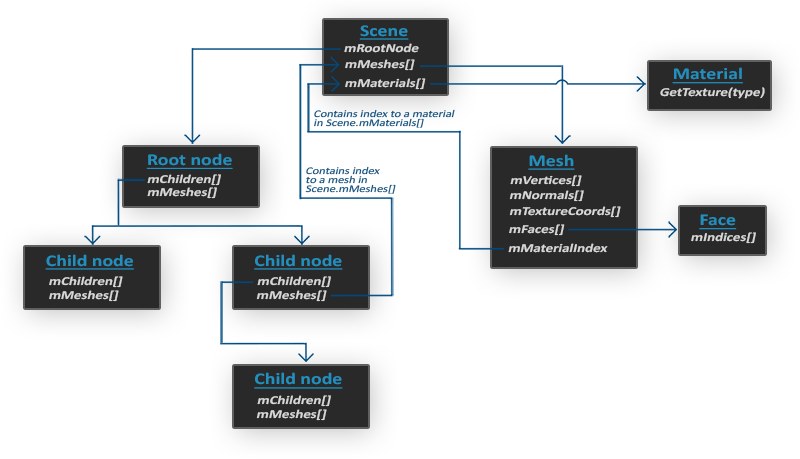
\includegraphics[width=\textwidth,height=\textheight,keepaspectratio]{Figures/Ch5/assimp_structure.png}}

	\caption{ساختار کلاس‌های کتابخانه‌ی \lr{Assimp} \cite{LearnOpenGL_Assimp}}
	\label{fig:Assimp}
  \end{figure}
  


  
\subsection{\lr{stb}}

این کتابخانه برای بارگذاری تصاویر استفاده می‌شود. در این پروژه از این کتابخانه برای بارگذاری
تصاویر بافت‌ها در کنار کتابخانه‌ی 
\lr{Assimp}
استفاده شده است.
\cite{stb}


\section{پیاده‌سازی}

این بخش دو هدف کلی را دنبال می‌کند.

\begin{enumerate}
	\item نمایش مدل گرافیکی و اجرای انیمیشن بر روی ‌آن
	\item ترکیب انیمیشن‌های مختلف به وسیله‌ی ماشین حالت

\end{enumerate}

\subsection{نمایش مدل گرافیکی}

همانطور که گفته شد مدل‌ها یا اشیاء سه‌بعدی به خودی خود مفهومی در 
\lr{OpenGL}
ندارند. آنچه برای 
\lr{OpenGL}
اهمیت دارد لیستی از مثلث‌ها است تا آن‌ها را به تصویر بکشد.
مدل‌های سه‌بعدی از رئوس، لبه و وجوه تشکیل می‌شوند و در فرمت‌های مختلفی مانند
\lr{FBX}
ذخیره می‌شوند. در این پیا‌ده‌سازی، از کتابخانه‌ی 
\lr{Assimp}
برای خواندن این داده‌ها استفاده شده است.

\subsection{قرارگیری مدل سه‌بعدی در کارت گرافیک}

آنچه برای 
\lr{OpenGL}
 اهمیت دارد این است که به آن مجموعه‌ای از مثلث‌ها داده شود تا برایمان ترسیم کند.
برای اینکار به صورت عمومی از 3 آرایه مختلف استفاده می‌شود که به نام‌های 
\lr{VBO}
،
\lr{VAO}
و 
\lr{EBO}
شناخته می‌شوند.
\lr{VBOs}
\LTRfootnote{Vertex Buffer Objectss}
یک آرایه یا بافری است که تمامی رئوس مدل سه‌بعدی ما را در خود جای می‌دهد.
همانطور که در بخش  2-2-1
اشاره شد، رئوس علاوه بر اینکه شامل اطلاعات موقعیت مکانی در محیط سه‌بعدی هستند، شامل اطلاعات دیگری 
نظیر رنگ، بردار نرمال، مختصات بافت  و... نیز می‌توانند باشند. بنابراین باید به صورتی به کارت گرافیک 
اعلام کنیم که این داده‌ای که در آرایه‌ی 
\lr{VBOs}
قرار دارد را چگونه تفسیر کند.
اینکار با استفاده از یک آرایه‌ی دیگر به نام 
\lr{VAO}
\LTRfootnote{Vertex Array Objects}
صورت می‌گیرد.
در نهایت گفتیم که آنچه برای کارت گرافیک اهمیت دارد دریافت مثلث‌ها است. بنابراین باید به طریقی بگوییم کدارم رئوس با 
اتصال به یکدیگر مثلث تشکیل می‌دهند. اینکار نیز با استفاده از آرایه‌ی 
\lr{EBOs}
\LTRfootnote{Element Buffer Objects}
صورت می‌گیرد.

\subsection{اسکلت شخصیت}

اسکلت یک شخصیت به صورت مجموعه‌ای از مفاصل که به صورت سلسله مراتبی به یکدگیر متصل‌اند، تعریف می‌شود.
در این پیاده‌سازی کلاس 
\lr{Bone}
نشان‌دهنده‌ی هر مفصل است.
هر 
\lr{Bone}
یک والد دارد و می‌تواند به هر تعدادی فرزند داشته باشد.
با توجه به تعریف آورده شده از اسکلت، کلاس اسکلت که با
\lr{Skeleton}
مشخص شده، شامل لیستی از این مفاصل به همراه اشاره‌گری به مفصل ریشه است.

\subsection{اتصال اسکلت و مدل سه‌بعدی}
اصطلاحی که برای اتصال اسکلت و مدل سه‌بعدی استفاده می‌شود
\lr{Skinning}
است.
در این روش هر راس موجود در مدل، به یک یا چند مفصل متصل می‌شود.
الگوریتم به کار‌رفته در این پیاده‌سازی،الگوریتم
\lr{linear blend skinning}
نام دارد. در این الگوریتم زمانی که یک راس به یک مفصل می‌شود به آن یک وزن نسبت داده می‌شود.
این وزن نشان‌دهنده‌ی میزان تاثیرگذاری این مفصل بر روی این راس است.
به بیانی دیگر، این وزن نشان می‌دهد که اکر این مفصل به مکان جدید منتقل شود، این انتقال چقدر بر روی آن راس تاثیر می‌گذارد.
بنابراین برای بدست آوردن انتقال نهایی راس، باید انتقال راس را نسبت به هرکدام از مفاصلی که به آن متصل است را بدست آوریم، سپس انتقال نهایی
برابر مجموع وزن‌دار تمامی این انتقال‌ها خواهد بود. 

\subsection{انیمیشن}
هر بازی‌های کامپیوتری هر کلیپ انیمیشنی شامل یک حرکت منحصر به فرد شخصیت داخل بازی است.
هر کلیپ‌ شامل ژست‌های اسکلت در فاصله‌های زمانی مشخصی است. در واقع آنچه باعث حرکت شخصیت می‌شود حرکت اسکلت شخصیت است.
زمانی که اسکلت شخصیت با استفاده از یک انیمیشن جابه‌جا می‌شود، مدل شخصیت نیز با استفاده از روش‌های 
\lr{skinning}
که در بالا توضیح داده‌شد همراه این اسکلت حرکت می‌کند.
انیمیشن‌ها از طریق کلاسی به اسم
\lr{Animation Clip}
مدل‌سازی شده اند. 
این کلاس شامل آرایه‌ای از ژست های شخصیت در مدت زمان‌های مشخصی است. همراه یک اشاره‌گری به اسکلت شخصیت.
نکته‌ی قابل توجه این است که هر کلیپ انیمیشنی مربوط به یک نوع اسکلت می‌شود. به زبانی دیگر نمی‌توان انیمیشنی که براس اسکلت
شخصیت انسانی طراحی شده است را بر روی یک حیوان، مانند فیل اجرا کرد.

\subsection{پخش‌کننده‌ی انیمیشن}

این سیستم وظیفه‌اش پخش کردن انیمیشن بر روی اسکلت شخصیت است.
این سیستم با گرفتن یک انیمیشن و یک اسکلت، این انیمیشن را بر روی آن اسکلت اجرا می‌کند.
همانطور که گفتیم، انیمیشن ها ژست شخصیت را در فاصله‌های زمانی مشخصی در خود ذخیره ‌می‌کنند. وظیفه‌ی این سیستم این است که با استفاده از یک زمان‌سنج که نشان‌دهنده‌ی زمان فعلی بازی است ژست مناسب شخصیت را از داخل انیمیشن بدست آورد.
قابل ذکر است که ممکن است این ژست با توجه به زمان بازی و فاصله‌های زمانی داخل انیمیشن
از درون‌یابی دو ژست پشت سر هم در آن کلیپ بدست آید.

\subsection{الگوریتم پخش‌کننده‌ی انیمیشن }

هر شخصیت درون بازی، اگر از نوع شخصیت اسکلتونی باشد، دارای یک پخش کننده ی انیمیشن خواهد بود.

در تصویر زیر تابع به‌روزرسانی اسکلت به وسیله‌ی انیمیشن را می‌توان مشاهده کرد.

\begin{latin}
	\begin{lstlisting}
		currentTime += deltaTime;

		const double currentAnimationTime = (currentTime - startTimeForCurrentAnim);
		AnimationPose currentPose = currentClip->GetPoseForCurrentFrame(currentAnimationTime * currentClip->GetFramePerSecond());
		
		SetSkeletonPose(currentPose);
	\end{lstlisting}
\end{latin}	



برای اینکه بتوان یک انیمیشن را پخش کرد نیاز است دو مورد زیر را بدانیم.

\begin{enumerate}
	\item زمان فعلی درون بازی(\lr{CurrentTime})
	\item زمان شروع پخش انیمیشن فعلی(\lr{StartTimeForCurrentAnimation}) 
\end{enumerate}

در ابتدا زمان فعلی درون بازی را برای این پخش‌کننده به‌روزرسانی می‌کنیم.
سپس برای بدست آوردن زمان فعلی انیمیشن می‌توان از فرمول زیر استفاده کرد

\lr{CurrentAnimationTime = CurrentTime - StartTimeForCurrentAnimation}

در نهایت با استفاده از این مقدار می‌توان ژست مورد نظر را از داخل کلیپ انیمیشنی بدست ‌آورد.
در نهایت نیز این ژست را بر روی اسکلت شخصیت اعمال می‌کنیم.


\subsection{ماشین حالت انیمیشن}

یکی از روش‌های ترکیب انیمیشن‌های مختلف با یکدیگر، استفاده از ماشین حالت متناهی است.
یک ماشین‌ حالت متناهی شامل چندی حالت مختلف است
که هر کدام از این حالات، حالتی از وضعیت سیستم را مشخص می‌کنند.
زمانی که از ماشین حالت استفاده می شود سیستم می‌تواند در هر لحظه تنها در یکی از این حالات قرار گیرد.
البته سیستم می‌تواند با دریافت ورودی از یک حالت به حالت دیگری رود.

دلیل استفاده از ماشین حالت متناهی برا سیستم انیمیشن این است که همانگونه که گفتیم، کلیپ‌های انیمیشنی، شامل ویدیو‌های کوتاهی هستند که یک حالت مشخصی از شخصیت را بیان می‌کنند.
در یک بازی، با توجه به ورودی بازیکن، شخصیت درون بازی می‌تواند در حالت‌های متفاوتی قرار گیرد. با استفاده از ماشین حالت می‌توان به تمامی این حالت‌ها رسیدگی کرد.

به عنوان مثال، تصویر زیر نشان‌دهنده‌ی یک ماشین‌حالت برای حرکت شخصیت است. شخصیت در ابتدا در حالت ایستاده قرار دارد و با گرفتن
ورودی‌های مختلف از کیبورد، می‌تواند به حالت‌های دیگری رود.

\begin{figure}[ht]
	\centerline{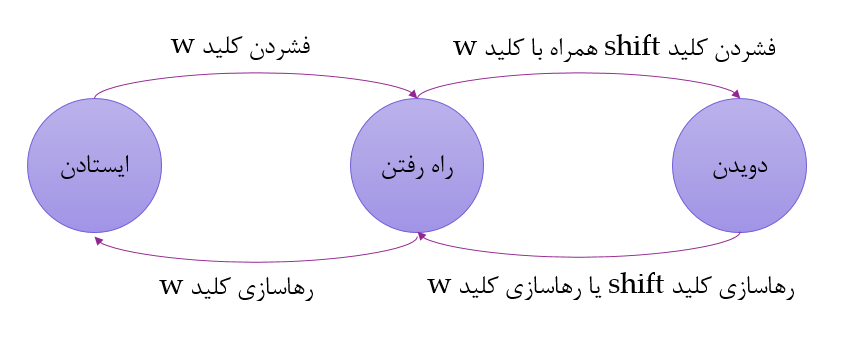
\includegraphics[width=\textwidth,height=\textheight,keepaspectratio]{Figures/Ch5/LocomotionStateMachine.png}}

	\caption{ماشین حالت برای حرکت شخصیت}
	\label{fig:LocomotionStateMachine}
\end{figure}


برای پیا‌ده‌سازی ماشین حالت متناهی، این سیستم به سه کلاس کلی شکسته‌شده‌است. کلاس
\lr{AnimationStateMachine}
که وظیفه‌ی مدیریت حالت‌ها و انتقال از یک حالت به حالت دیگری را دارد.
کلاس 
\lr{AnimationState}
که نشان‌دهنده‌ی حالت شخصیت است. هر 
\lr{AnimationState}
شامل یک کلیپ است و هر زمانی که این حالت فعال می‌شود این کلیپ پخش می‌شود.
 در نهایت کلاس
\lr{Transition}
که شامل توابع انتقال است.
هر حالت می‌تواند شامل چندین انتقال باشد. و وظیفه‌ی
\lr{AnimationStateMachine}
است که بررسی کند، اگر انتقالی امکان‌پذیر بود، آن را انجام دهد.

\subsection{به‌روزرسانی ماشین حالت انیمیشن}

وضعیت توابع انتقال تاثیرگذاری مستقیمی در وضعیت سیستم به‌روزرسانی ماشین حالت انیمیشن دارد.
وضعیت انتقال می‌تواند سه حالت زیر را داشته باشد.

\begin{enumerate}
	\item حالت عادی \LTRfootnote{Normal}
	\item حالت در حال انتقال \LTRfootnote{Transitioning}
	\item حالت اتمام انتقال \LTRfootnote{Finished}
\end{enumerate}


حالت اول حالت عادی
است که نشان‌دهنده‌ی وضعیت عادی ماشین حالت است. در این وضعیت، توابع انتقال حالت فعلی بررسی می‌شوند تا در صورتی که شرایطشان برقرار شود، تغییر حالت رخ دهد. علاوه بر آن انیمیشن حالت فعلی با استفاده از کلاس پخش‌کننده آپدیت می‌شود.
در صورتی که توابع انتقال مقدار درست
\LTRfootnote{True}
را بازگردانند، ماشین به وضعیت دوم که وضعیت درحال انتقال
است، تغییر وضعیت می‌دهد.
در این وضعیت با توجه به زمانی که مشخص شده، ژست شخصیت با استفاده از درون‌یابی خطی از حالت فعلی به حالت جدید تغییر می‌کند.
پس از اینکه انتقال به صورت کامل انجام شد، وضعیت ماشین حالت به اتمام انتقال
تغییر می‌یابد. زمانی که ماشین‌ در این وضعیت قرار گرفته یعنی به حالت جدید منتقل شده، بنابراین لازم است انیمیشن را از حالت جدید گرفته و آن را به کلاس پخش کننده داده تا آن را پخش کند.
پس از این کار وضعیت ماشین دوباره به حالت عادی تغییر می‌یابد و همه‌ی این موارد دوباره تکرار می‌شوند.

\begin{latin}
	

\begin{lstlisting}

	if(transitionStatus == TransitionStatus::normal) 
	{
		for (const auto&  transition : currentState->GetTransitions()) // loop through transitions of the current state
		{
			if (transition->Evaluate())
			{
				transitionStatus = TransitionStatus::transitioning;
				currentState = animationStatesMap.at(transition->to);
				TransitionFromPose = animator->GetPoseAtCurrentTime();
				TransitionToPose = currentState->GetAnimClip()->GetPoseForCurrentFrame(0);
				currentTime = 0;
				transitionTime = transition->transitionTime;
				break;
			}
		}
	}

	if (transitionStatus == TransitionStatus::normal)
	{
		animator->Update(deltaTime);
	}
	else if(transitionStatus == TransitionStatus::transitioning)
	{
		if(TransitionUpdate(deltaTime)) 
		{
			transitionStatus = TransitionStatus::finished;
		}
	}
	else if(transitionStatus == TransitionStatus::finished)
	{
		animator->ChangeAnimationClip(*(currentState->GetAnimClip()), 0); 
		transitionStatus = TransitionStatus::normal;
	}
\end{lstlisting}

\end{latin}
\chapter {نتیجه‌گیری }

هدف این پروژه آشنایی با محیط‌های گرافیکی و الگوریتم‌های موجود در آن با 
تاکید بر سیستم پویانمایی کامپیوتری بود.
برای بدست آوردن این هدف، در این پروژه ابتدا به بررسی سیستم گراف 
پویانمایی یکی از بزرگترین موتور‌های بازی‌سازی جهان، یعنی موتور بازی‌سازی آنریل 
پرداختیم.
با این بررسی متوجه‌‌شدیم که یک سیستم پویانمایی چه ابزارهایی را در اختیار کاربران 
قرار می‌دهد و نحوه‌ی کلی استفاده از این ابزار‌ها چگونه است.

در نهایت برای تحلیل عمیق این سیستم‌ها به پیاده‌سازی یک سیستم مشابه 
با استفاده از واسط برنامه نویسی کاربردی 
\lr{OpenGL}
پرداختیم.
خروجی این پیاده‌سازی، یک نرم‌افزاری گرافیکی است که به وسیله‌ی آن 
می‌توان مش‌های اسکلتی را بارگذاری کرد و روی آن‌ها کلیپ‌های 
پویانمایی مختلفی را اجرا کرد.

\chapter {کار‌‌های آینده}

نرم‌افزار گرافیکی پیاده‌سازی شده می‌تواند از جهات مختلفی گسترش یابد.
 یکی از مواردی که می‌توان اشاره کرد 
ایجاد ویژگی‌های جدید به نرم‌افزار فعلی است. همانطور که در تحقیق درباره‌ی سیستم آنریل متوجه‌ شدیم، سیستم‌‌های پویانمایی،
سیستم‌‌های بسیار گسترده‌ای هستند. ویژگی‌هایی مانند، اضافه کردن الگوریتم‌های مختلف برای ترکیب،
اضافه کردن پویانمایی بر اساس فیزیک، اضافه کردن 
مواردی همچون سینماتیک معکوس برای ایجاد پویانمایی رویه‌ای می‌توانند تنها سطحی از دریای عمیق ویژگی‌ها باشند.

علاوه بر این، از آنجایی که این برنامه‌ی در حال حاضر از کتابخانه‌ی 
\lr{Assimp}
برای بارگذاری مدل‌های سه‌بعدی استفاده می‌کند، سرعت مناسبی ندارد.
می‌توان با نوشتن یک سیستم جداگانه برای بارگذاری اشیاء به سرعت این بارگذاری افزود.

علاوه بر این موارد، این برنامه را می‌توان از جهت موتور بازی‌سازی نیز ارتقا بخشید.
به عنوان مثال، در سیستم فعلی هیچگونه الگوریتم برخوردی، پیاده‌سازی نشده است. با پیاده‌سازی چنین مواردی،
می‌توان به واقع‌گرایانه‌تر شدن این برنامه کمک کرد.
%\chapter{امتحانی}
\section{نمرات}
سلام سلام سلام%
\LTRfootnote{hello}
\LTRfootnote{hi}
\begin{itemize}
	\item یک
	\item دو
\end{itemize}

\%13 

\begin{equation}
\frac{1}{2}
\end{equation}

$2$

مرجع های 
\cite{Amintoosi09regional,Baker02limits}

%%%%%%%%%%%%%%%%%%%%%%%%%%%%%%%%%%%%%%%%%%%%%%%%%%%%%
\chapter{آشنایی سریع با برخی دستورات لاتک}\label{Chap:latexIntro}
در این فصل ویژگی‌های مهم و پرکاربرد زی‌پرشین و لاتک معرفی می‌شود. برای راهنمایی بیشتر و به‌کاربردن ویژگی‌های پیشرفته‌تر به راهنمای زی‌پرشین و راهنمای لاتک مراجعه کنید. برای آگاهی از دستورات لاتک که این خروجی را تولید کرده‌اند فایل \lr{Chapter2.tex} را ملاحظه فرمایید.
\footnote{بیشتر مطالب این بخش از مثال 
	\lr{xepersian\_example.tex}
	گرفته شده‌اند که توسط دوستمان آقای امیرمسعود پورموسی آماده شده بوده است.}

\section{بندها و زیرنویس‌ها}
هر جایی از نوشته خود، اگر می‌خواهید به سر سطر بروید و یک بند تازه را آغاز کنید، باید یک خط را خالی بگذارید
\footnote{یعنی دوبار باید کلید \lr{Enter} را بزنید.}
مانند این:

حالا که یک بند تازه آغاز شده است، یک زیرنویس انگلیسی
\LTRfootnote{English Footnote!}
هم می‌نویسیم!
\section{فرمول‌های ریاضی}\label{formula}

اینجا هم یک فرمول می‌آوریم که شماره دارد:
\begin{equation}\label{eq:yek}
A=\frac{c}{d}+\frac{q^2}{\sin(\omega t)+\Omega_{12}}
\end{equation}
در لاتک می‌توان به کمک فرمان 
\lr{\textbackslash label\{\}}
به هر فرمول یک نام نسبت داد. در فرمول بالا نام \lr{eq:yek} را برایش گذاشته‌ایم (پرونده \lr{tex} همراه با این مثال را ببینید). این نام ما را قادر می‌کند که بعداً بتوانیم با فرمان
\lr{\textbackslash ref\{eq:yek\}}
به آن فرمول با شماره ارجاع دهیم. یعنی بنویسیم فرمول \ref{eq:yek}. 
لاتک خودش شماره این فرمول‌ها را مدیریت می‌کند.\footnote{یعنی اگر بعداً فرمولی قبل از این فرمول بنویسیم، خودبه‌خود شماره این فرمول و شماره ارجاع‌ها به این فرمول یکی زیاد می‌شود. دیگر نگران شماره‌گذاری فرمول‌های خود نباشید!} این هم یک فرمول که شماره ندارد:
$$A=|\vec{a}\times \vec{b}| + \sum_{n=0}^\infty C_{ij}$$

این هم عبارتی ریاضی مانند 
$\sqrt{a^2+b^2}$
که بین متن می‌آید.
\subsection{یک زیربخش}\label{zirbakhsh}

این زیربخش \ref{zirbakhsh} است؛ یعنی یک بخش درون بخش \ref{formula} است.
\subsubsection{یک زیرزیربخش}
این هم یک زیرزیربخش است. در لاتک می‌توانید بخش‌های تودرتو در نوشته‌تان تعریف کنید تا ساختار منطقی نوشته را به خوبی نشان دهید. می‌توانید به این بخش‌ها هم با شماره ارجاع دهید، مثلاً بخش فرمول‌های ریاضی شماره‌اش \ref{formula} است.
\section{نوشته‌های فارسی و انگلیسی مخلوط}
نوشتن یک کلمه انگلیسی بین متن فارسی بدیهی است، مانند 
\lr{Example}
در این جمله.
نوشتن یک عبارت چندکلمه‌ای مانند
\lr{More than one word} کمی پیچیده‌تر است.

اگر ناگهان تصمیم بگیرید که یک بند کاملاً انگلیسی را بنویسید، باید:
\begin{latin}
	This is an English paragraph from left to right. You can write as much as you want in it.
\end{latin}
\section{افزودن تصویر به نوشته}
پرونده تصویر دلخواه خود را در کنار پرونده \lr{tex} قرار دهید. سپس به روش زیر تصویر را در نوشته خود بیاورید:
\begin{latin}
	\begin{verbatim}
	\includegraphics{YourImageFileName}
	\end{verbatim}
\end{latin}
به تصویرها هم مانند فرمول‌ها و بخش‌ها می‌توان با شماره ارجاع داد. مثلاً تصویر  \ref{fig:shir} یک شیر علاقه‌مند به لاتک را در حال دویدن نشان می‌دهد. برای جزئیات بیشتر درباره روش گذاشتن تصویرها در نوشته باید راهنماهای لاتک را بخوانید.
\begin{figure}%[ht]
	\centerline{
\includegraphics[width=5cm]{Figures/Ch2/lion.jpg}}
	\caption{در این تصویر یک شیر علاقه‌مند به لاتک را در حال دویدن می‌بینید.}
	\label{fig:shir}
\end{figure}

به تصویرها هم مانند فرمول‌ها و بخش‌ها می‌توان با شماره ارجاع داد. مثلاً تصویر بالا شماره‌اش \ref{fig:shir} است. برای جزئیات بیشتر درباره روش گذاشتن تصویرها در نوشته باید راهنماهای لاتک را بخوانید.

\section{محیط‌های شمارش و نکات}
برای فهرست‌کردن چندمورد، اگر ترتیب برایمان مهم نباشد:
\begin{itemize}
	\item[-] مورد یکم
	\item[-] مورد دوم
	\item[-] مورد سوم
\end{itemize}
و اگر ترتیب برایمان مهم باشد:
\begin{enumerate}
	\item مورد یکم
	\item مورد دوم
	\item مورد سوم
\end{enumerate}
می‌توان موردهای تودرتو داشت:
\begin{enumerate}
	\item مورد ۱
	\item مورد ۲
	\begin{enumerate}
		\item مورد ۱ از ۲
		\item مورد ۲ از ۲
		\item مورد ۳ از ۲
	\end{enumerate}
	\item مورد ۳
\end{enumerate}
شماره‌گذاری این موردها را هم لاتک انجام می‌دهد.
%\section{تعریف و قضیه}
%برای ذکر تعریف، قضیه و مثال مثالهای ذیل را ببینید.
%\begin{definition}
%	مجموعه همه ارزیابی‌های  (پیوسته)  روی $(X,\tau)$، دامنه توانی احتمالی
%	\index{دامنه توانی احتمالی}
%	$ X $
%	نامیده می‌شود.
%\end{definition}
%\begin{theorem}[باناخ-آلااغلو]
%	\index{قضیه باناخ-آلااغلو}
%	اگر $ V $ یک همسایگی $ 0 $ در فضای برداری 
%	\index{فضای!برداری}
%	توپولوژیکی $ X $ باشد و 
%	\begin{equation}\label{eq1}
%	K=\left\lbrace \Lambda \in X^{*}:|\Lambda x|\leqslant 1 ; \ \forall x\in V\right\rbrace,
%	\end{equation}
%	آنگاه $ K $،  ضعیف*-فشرده است که در آن، $ X^{*} $ دوگان
%	\index{فضای!دوگان}
%	فضای برداری توپولوژیکی $ X $ است به ‌طوری که عناصر آن،  تابعی‌های 
%	خطی پیوسته
%	\index{تابعی خطی پیوسته}
%	روی $X$ هستند.
%\end{theorem}
%تساوی \eqref{eq1} یکی از مهم‌ترین تساوی‌ها در آنالیز تابعی است که در ادامه، به وفور از آن استفاده می‌شود.
%\begin{example}
%	برای هر فضای مرتب، گردایه 
%	$$U:=\left\lbrace U\in O: U=\uparrow U\right\rbrace $$
%	از مجموعه‌های بالایی باز، یک توپولوژی تعریف می‌کند که از توپولوژی اصلی، درشت‌تر  است.
%\end{example}
%حال تساوی 
%\begin{equation}\label{eq2}
%\sum_{n=1}^{+\infty} 3^{n}x+7x=\int_{1}^{n}8nx+\exp{(2nx)}
%\end{equation}
%را در نظر بگیرید. با مقایسه تساوی \eqref{eq2} با تساوی \eqref{eq1} می‌توان نتیجه گرفت که ...
%
\section{چگونگی نوشتن و ارجاع به مراجع}\label{Sec:Ref}

در لاتک به راحتی می‌توان مراجع خود را نوشت و به آنها ارجاع داد. به عنوان مثال برای معرفی کتاب گنزالس \cite{Gonzalez02book} به عنوان یک مرجع می‌توان آنرا به صورت زیر معرفی نمود:

\singlespacing
\begin{LTR}
	\begin{verbatim}
	\bibitem{Gonzalez02book}
	Gonzalez, R.C., and Woods, R.E. {\em Digital Image Processing}, 3rd ed..
	Prentice-Hall, Inc., Upper Saddle River, NJ, USA, 2006.
	\end{verbatim}
\end{LTR}
\doublespacing

در دستورات فوق \lr{Gonzalez02book}  برچسبی است که به این مرجع داده شده است و با استفاده از دستور 
\verb!\cite{Gonzalez02book}!
می‌توان به آن ارجاع داد؛ بدون این که شماره‌اش را در فهرست مراجع‌مان بدانیم.

اگر این اولین مرجع ما باشد در قسمت مراجع به صورت زیر خواهد آمد:\\
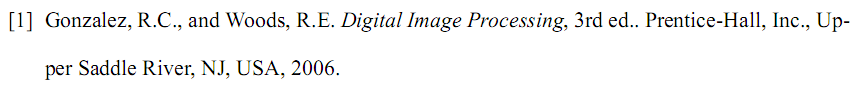
\includegraphics[width=\textwidth]{Figures/Ch2/gonzalez.png}

این شیوه برای تعداد مراجع کم بد نیست اما اگر فرمت مراجع، ترتیب یا تعداد آنها را خواسته باشید تغییر دهید، به عنوان مثال ابتدا حرف اول نام نویسنده بیاید و سپس نام خانوادگی، باید همه کارها را به صورت دستی انجام دهید.
اگر مایلید کنترل کاملی بر مراجع خود داشته باشید و به راحتی بتوانید قالب مراجع خود را عوض کنید باید از \lr{Bib\TeX} استفاده کنید که درپیوست  \ref{App:RefMan} به  آن پرداخته خواهد شد.



% ░░░░░░░▒▒▒▒▒▒▓▓▓▓ Appendices ▓▓▓▓▒▒▒▒▒▒░░░░░░░
%\MakeAppendices%
%\section{مدیریت مراجع در لاتک}\label{App:RefMan}
در بخش \ref{Sec:Ref} اشاره شد که با دستور 
 \lr{\textbackslash bibitem}
  می‌توان یک مرجع را تعریف نمود و با فرمان
 \lr{\textbackslash cite}
  به آن ارجاع داد. این روش برای تعداد مراجع زیاد و تغییرات آنها مناسب نیست. در ادامه به صورت مختصر توضیحی در خصوص برنامه \lr{BibTeX} که همراه با توزیع‌های معروف تِک عرضه می‌شود و نحوه استفاده از آن در زی‌پرشین خواهیم داشت.

\subsection{ مدیریت مراجع با  \texorpdfstring{\lr{Bib\TeX}}{Bib\TeX} }
یکی از روش‌های قدرتمند و انعطاف‌پذیر برای نوشتن مراجع مقالات و مدیریت مراجع در لاتک، استفاده از  \lr{BibTeX} است.
 روش کار با  \lr{BibTeX} به این صورت است که مجموعه‌ی همه‌ی مراجعی را که در پروژه/پایان‌نامه/رساله استفاده کرده یا خواهیم کرد، 
در پرونده‌ی جداگانه‌ای نوشته و به آن فایل در سند خودمان به صورت مناسب لینک می‌دهیم.
 کنفرانس‌ها یا مجله‌های گوناگون برای نوشتن مراجع، قالب‌ها یا قراردادهای متفاوتی دارند که به آنها استیلهای مراجع گفته می‌شود.
 در این حالت به کمک ‌استیل‌های \lr{BibTeX} خواهید توانست تنها با تغییر یک پارامتر در پرونده‌ی ورودی خود، مراجع را مطابق قالب موردنظر تنظیم کنید. 
 بیشتر مجلات و کنفرانس‌های معتبر یک پرونده‌ی سبک (\lr{BibTeX Style}) با پسوند \lr{bst} در وب‌گاه خود می‌گذارند که برای همین منظور طراحی شده است.

به جز نوشتن مقالات این سبک‌ها کمک بسیار خوبی برای تهیه‌ی مستندات علمی همچون پایان‌نامه‌هاست که فرد می‌تواند هر قسمت از کارش را که نوشت مراجع مربوطه را به بانک مراجع خود اضافه نماید. با داشتن چنین بانکی از مراجع، وی خواهد توانست به راحتی یک یا چند ارجاع به مراجع و یا یک یا چند بخش را حذف یا اضافه ‌نماید؛ 
مراجع به صورت خودکار مرتب شده و فقط مراجع ارجاع داده شده در قسمت کتاب‌نامه خواهندآمد. قالب مراجع به صورت یکدست مطابق سبک داده شده بوده و نیازی نیست که کاربر درگیر قالب‌دهی به مراجع باشد. 
در این جا مجموعه‌ سبک‌های بسته \lr{Persian-bib} که برای  زی‌پرشین آماده شده‌اند به صورت مختصر معرفی شده و روش کار با آن‌ها گفته می‌شود. برای اطلاع بیشتر به راهنمای بسته‌ی \lr{Persian-bib} مراجعه فرمایید.
\subsection{سبک‌های فعلی قابل استفاده در زی‌پرشین}
در حال حاضر فایلهای سبک زیر برای استفاده در زی‌پرشین آماده شده‌اند:

\singlespacing
\begin{description}
\item [\lr{unsrt-fa.bst}] این سبک متناظر با \lr{unsrt.bst} می‌باشد. مراجع به ترتیب ارجاع در متن ظاهر می‌شوند.
\item [\lr{plain-fa.bst}] این سبک متناظر با \lr{plain.bst} می‌باشد. مراجع بر اساس نام‌خانوادگی نویسندگان، به ترتیب صعودی مرتب می‌شوند.
 همچنین ابتدا مراجع فارسی و سپس مراجع انگلیسی خواهند آمد.
\item [\lr{acm-fa.bst}] این سبک متناظر با \lr{acm.bst} می‌باشد. شبیه \lr{plain-fa.bst} است.  قالب مراجع کمی متفاوت است. اسامی نویسندگان انگلیسی با حروف بزرگ انگلیسی نمایش داده می‌شوند. (مراجع مرتب می‌شوند)
\item [\lr{ieeetr-fa.bst}] این سبک متناظر با \lr{ieeetr.bst} می‌باشد. (مراجع مرتب نمی‌شوند)
\item [\lr{plainnat-fa.bst}] این سبک متناظر با \lr{plainnat.bst} می‌باشد. نیاز به بسته \lr{natbib} دارد. (مراجع مرتب می‌شوند)
\item [\lr{chicago-fa.bst}] این سبک متناظر با \lr{chicago.bst} می‌باشد. نیاز به بسته \lr{natbib} دارد. (مراجع مرتب می‌شوند)
\item [\lr{asa-fa.bst}] این سبک متناظر با \lr{asa.bst} می‌باشد. نیاز به بسته \lr{natbib} دارد. (مراجع مرتب می‌شوند)
\item[\lr{ModifiedIEEEtranFa.bst}] این سبک متناظر با نحوه ارجاع در پایان‌نامه‌های دانشگاه صنعتی اصفهان می‌باشد.
\end{description}
\doublespacing

با استفاده از استیلهای فوق می‌توانید به انواع مختلفی از مراجع فارسی و لاتین ارجاع دهید. به عنوان نمونه مرجع 
\cite{Omidali82phdThesis}
 یک نمونه پروژه دکترا (به فارسی) و مرجع 
\cite{Vahedi87} یک نمونه مقاله مجله فارسی است.
مرجع 
\cite{Amintoosi87afzayesh}  یک نمونه  مقاله کنفرانس فارسی و
مرجع 
\cite{Pedram80osool} یک نمونه کتاب فارسی با ذکر مترجمان و ویراستاران فارسی است. مرجع 
\cite{Khalighi07MscThesis} یک نمونه پروژه کارشناسی ارشد انگلیسی و
\cite{Khalighi87xepersian} هم یک نمونه متفرقه  می‌باشند.
مراجع 
\cite{Gonzalez02book,Baker02limits} 
نمونه کتاب و مقاله انگلیسی هستند.

استیل مورد استفاده در این پروژه/پایان‌نامه/رساله 
\lr{ModifiedIEEEtranFa}
است که خروجی آنرا در بخش مراجع می‌توانید مشاهده کنید.
نمونه  خروجی سبک \lr{asa-fa} در شکل \ref{fig:asafa} آمده است.

\begin{figure}[t]
\centering
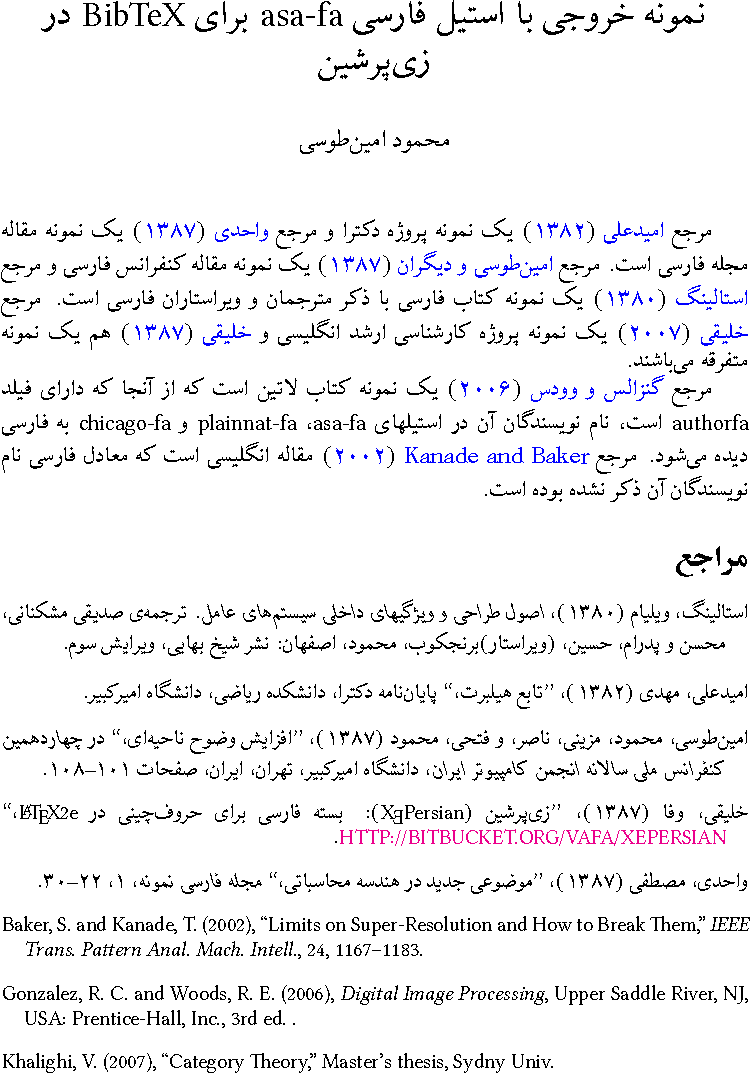
\includegraphics[width=.8\textwidth]{Figures/App1/asa-fa-crop.pdf}
\caption{نمونه خروجی با سبک \lr{asa-fa}}
\label{fig:asafa}
\end{figure} 
\subsection{ نحوه استفاده از سبک‌های فارسی}
برای استفاده از بیب‌تک باید مراجع خود را در یک فایل با پسوند \lr{bib} ذخیره نمایید. یک فایل \lr{bib} در واقع یک پایگاه داده از مراجع\LTRfootnote{Bibliography Database}  شماست که هر مرجع در آن به عنوان یک رکورد از این پایگاه داده
با قالبی خاص ذخیره می‌شود. به هر رکورد یک مدخل\LTRfootnote{Entry} گفته می‌شود. یک نمونه مدخل برای معرفی کتاب \lr{Digital Image Processing} در ادامه آمده است:

\singlespacing
\begin{LTR}
\begin{verbatim}
@BOOK{Gonzalez02image,
  AUTHOR =      {Rafael Gonzalez and Richard Woods},
  TITLE =       {Digital Image Processing},
  PUBLISHER =   {Prentice-Hall, Inc.},
  YEAR =        {2006},
  EDITION =     {3rd},
  ADDRESS =     {Upper Saddle River, NJ, USA}
}
\end{verbatim}
\end{LTR}
\doublespacing

در مثال فوق، \lr{@BOOK} مشخصه‌ی شروع یک مدخل مربوط به یک کتاب و \lr{Gonzalez02book} برچسبی است که به این مرجع منتسب شده است.
 این برچسب بایستی یکتا باشد. برای آنکه فرد به راحتی بتواند برچسب مراجع خود را به خاطر بسپارد و حتی‌الامکان برچسب‌ها متفاوت با هم باشند معمولاً از قوانین خاصی به این منظور استفاده می‌شود. یک قانون می‌تواند فامیل نویسنده‌ی اول+دورقم سال نشر+اولین کلمه‌ی عنوان اثر باشد. به \lr{AUTHOR} و $\dots$ و \lr{ADDRESS} فیلدهای این مدخل گفته می‌شود؛ که هر یک با مقادیر مربوط به مرجع مقدار گرفته‌اند. ترتیب فیلدها مهم نیست. 

انواع متنوعی از مدخل‌ها برای اقسام مختلف مراجع همچون کتاب، مقاله‌ی کنفرانس و مقاله‌ی ژورنال وجود دارد که برخی فیلدهای آنها با هم متفاوت است. 
نام فیلدها بیانگر نوع اطلاعات آن می‌باشد. مثالهای ذکر شده در فایل \lr{References.bib} کمک خوبی به شما خواهد بود. 
%این فایل یک فایل متنی بوده و با ویرایشگرهای معمول همچون \lr{Notepad++} قابل ویرایش می‌باشد. برنامه‌هایی همچون 
%\lr{TeXMaker}
% امکاناتی برای نوشتن این مدخل‌ها دارند و به صورت خودکار فیلدهای مربوطه را در فایل \lr{bib}  شما قرار می‌دهند.  
با استفاده از سبک‌های فارسی آماده شده، محتویات هر فیلد می‌تواند به فارسی نوشته شود، ترتیب مراجع و نحوه‌ی چینش فیلدهای هر مرجع را سبک مورد استفاده  مشخص خواهد کرد.

نکته: بدون اعمال تنظیمات موردنیاز \lr{Bib\TeX} در \lr{TeXWorks}، مراجع فارسی در استیل‌هایی که مراجع را به صورت مرتب شده چاپ می‌کنند، ترتیب کاملاً درستی نخواهند داشت. برای توضیحات بیشتر \cite{persianbib87userguide} را ببینید یا به سایت پارسی‌لاتک مراجعه فرمایید.

\textbf{برای درج مراجع خود لازم نیست نگران موارد فوق باشید. در فایل 
\lr{References.bib}
 که همراه با این پروژه/پایان‌نامه/رساله هست، موارد مختلفی درج شده است و کافیست مراجع خود را جایگزین موارد مندرج در آن نمایید.
}

پس از قرار دادن مراجع خود، یک بار \lr{XeLaTeX} را روی سند خود اجرا نمایید، سپس \lr{bibtex} و پس از آن دوبار \lr{XeLaTeX} را. در \lr{TeXstudio} کلید \lr{F8} و در \lr{TeXWorks} هم گزینه‌ی \lr{BibTeX} از منوی \lr{Typeset}، \lr{BibTeX} را روی سند شما اجرا می‌کنند.

برای بسیاری از مقالات لاتین حتی لازم نیست که مدخل مربوط به آنرا خودتان بنویسید. با جستجوی نام مقاله + کلمه \lr{bibtex}  در اینترنت سایتهای بسیاری همچون \lr{ACM} و \lr{ScienceDirect} را خواهید یافت که مدخل \lr{bibtex} مربوط به مقاله شما را دارند و کافیست آنرا به انتهای فایل \lr{References} اضافه کنید.

از هر یک از سبکهای \lr{Persian-bib} می‌توانید استفاده کنید، البته اگر از سه استیل آخر استفاده می‌کنید و مایلید که مراجع شما شماره بخورند باید بسته \lr{natbib} را با گزینه \lr{numbers} فراخوانی نمایید.
\newpage
\section{‌جدول، نمودار و الگوریتم در لاتک}\label{App:Latex:More}
در این بخش نمونه مثالهایی از جدول، نمودار و الگوریتم در لاتک را خواهیم دید.
\subsection{مدلهای حرکت دوبعدی}
بسیاری از اوقات حرکت بین دو تصویر از یک صحنه با یکی از مدلهای پارامتری ذکر شده در جدول \eqref{tab:MotionModels} قابل مدل نمودن می‌باشد.  
\begin{table}[ht]
	\caption{مدلهای تبدیل.}
	\label{tab:MotionModels}
	\centering
	\onehalfspacing
	\begin{tabular}{|r|c|l|r|}
		\hline نام مدل & درجه آزادی & تبدیل مختصات & توضیح \\ 
		\hline انتقالی & ۲ & $\begin{aligned} x'=x+t_x \\ y'=y+t_y \end{aligned}$  &  انتقال دوبعدی\\ 
		\hline اقلیدسی & ۳ & $\begin{aligned} x'=xcos\theta - ysin\theta+t_x \\ y'=xsin\theta+ycos\theta+t_y \end{aligned}$  &  انتقالی+دوران \\ 
		\hline مشابهت & ۴ & $\begin{aligned} x'=sxcos\theta - sysin\theta+t_x \\ y'=sxsin\theta+sycos\theta+t_y  \end{aligned}$  & اقلیدسی+تغییرمقیاس \\ 
		\hline آفین & ۶ & $\begin{aligned} x'=a_{11}x+a_{12}y+t_x \\ y'=a_{21}x+a_{22}y+t_y \end{aligned}$  & مشابهت+اریب‌شدگی \\ 
		\hline  پروجکتیو & ۸ & $\begin{aligned} x'&=(m_1x+m_2y+m_3)/D \\ y'&=(m_4x+m_5y+m_6)/D \\ D&=m_7x+m_8y+1 \end{aligned}$  & آفین+\lr{keystone+chirping} \\ 
		\hline  شارنوری & $\infty $ & $\begin{aligned} x'=x+v_x(x,y) \\ y'=y+v_y(x,y) \end{aligned}$  &  حرکت آزاد\\ 
		\hline 
	\end{tabular} 
\end{table}

\subsection{ماتریس}

شناخته‌شده‌ترین روش تخمین ماتریس هوموگرافی الگوریتم تبدیل خطی مستقیم (\lr{DLT\LTRfootnote{Direct Linear Transform}}) است.  فرض کنید چهار زوج نقطهٔ متناظر در دو تصویر در دست هستند،  $\mathbf{x}_i\leftrightarrow\mathbf{x}'_i$   و تبدیل با رابطهٔ
$\mathbf{x}'_i = H\mathbf{x}_i$
نشان داده می‌شود که در آن:
\[\mathbf{x}'_i=(x'_i,y'_i,w'_i)^\top  \]
و
\[ H=\left[
\begin{array}{ccc}
h_1 & h_2 & h_3 \\ 
h_4 & h_5 & h_6 \\ 
h_7 & h_8 & h_9
\end{array} 
\right]\]
رابطه زیر را برای الگوریتم  \eqref{alg:DLT} لازم دارم.
\begin{equation}\label{eq:DLT_Ah}
\left[
\begin{array}{ccc}
0^\top & -w'_i\mathbf{x}_i^\top & y'_i\mathbf{x}_i^\top \\ 
w'_i\mathbf{x}_i & 0^\top & -x'_i\mathbf{x}_i^\top \\ 
- y'_i\mathbf{x}_i^\top & x'_i\mathbf{x}_i^\top & 0^\top
\end{array} 
\right]
\left(
\begin{array}{c}
\mathbf{h}^1 \\ 
\mathbf{h}^2 \\ 
\mathbf{h}^3
\end{array} 
\right)=0
\end{equation}

\subsection{الگوریتم با دستورات فارسی}
با مفروضات فوق، الگوریتم \lr{DLT} به صورت نشان داده شده در الگوریتم \eqref{alg:DLT}  خواهد بود.
\begin{algorithm}[t]
	\onehalfspacing
	\caption{الگوریتم \lr{DLT} برای تخمین ماتریس هوموگرافی.} \label{alg:DLT}
	\begin{algorithmic}[1]
		\REQUIRE $n\geq4$ زوج نقطهٔ متناظر در دو تصویر 
		${\mathbf{x}_i\leftrightarrow\mathbf{x}'_i}$،\\
		\ENSURE ماتریس هوموگرافی $H$ به نحوی‌که: 
		$\mathbf{x}'_i = H \mathbf{x}_i$.
		\STATE برای هر زوج نقطهٔ متناظر
		$\mathbf{x}_i\leftrightarrow\mathbf{x}'_i$ 
		ماتریس $\mathbf{A}_i$ را با استفاده از رابطهٔ \ref{eq:DLT_Ah} محاسبه کنید.
		\STATE ماتریس‌های ۹ ستونی  $\mathbf{A}_i$ را در قالب یک ماتریس $\mathbf{A}$ ۹ ستونی ترکیب کنید. 
		\STATE تجزیهٔ مقادیر منفرد \lr{(SVD)}  ماتریس $\mathbf{A}$ را بدست آورید. بردار واحد متناظر با کمترین مقدار منفرد جواب $\mathbf{h}$ خواهد بود.
		\STATE  ماتریس هوموگرافی $H$ با تغییر شکل $\mathbf{h}$ حاصل خواهد شد.
	\end{algorithmic}
\end{algorithm}

\subsection{الگوریتم با دستورات لاتین}
الگوریتم \ref{alg:RANSAC} یک الگوریتم با دستورات لاتین است.

\begin{algorithm}[t]
	\onehalfspacing
	\caption{الگوریتم \lr{RANSAC} برای تخمین ماتریس هوموگرافی.} \label{alg:RANSAC}
	\begin{latin}
		\begin{algorithmic}[1]
			\REQUIRE $n\geq4$ putative correspondences, number of estimations, $N$, distance threshold $T_{dist}$.\\
			\ENSURE Set of inliers and Homography matrix $H$.
			\FOR{$k = 1$ to $N$}
			\STATE Randomly choose 4 correspondence,
			\STATE Check whether these points are colinear, if so, redo the above step
			\STATE Compute the homography $H_{curr}$ by DLT algorithm from the 4 points pairs,
			\STATE $\ldots$ % الگوریتم کامل نیست
			\ENDFOR
			\STATE Refinement: re-estimate H from all the inliers using the DLT algorithm.
		\end{algorithmic}
	\end{latin}
\end{algorithm}

\subsection{نمودار}
لاتک بسته‌هایی با قابلیت‌های زیاد برای رسم انواع مختلف نمودارها دارد. مانند بسته‌های \lr{Tikz} و  \lr{PSTricks}. توضیح اینها فراتر از این پیوست کوچک است. مثالهایی از رسم نمودار را در مجموعه پارسی‌لاتک خواهید یافت. توصیه می‌کنم که حتماً مثالهایی از برخی از آنها را ببینید. راهنمای همه آنها در تک‌لایو هست. نمونه مثالهایی از بسته \lr{Tikz} را می‌توانید در \url{http://www.texample.net/tikz/examples/} ببینید.

\subsection{تصویر}
نمونه تصاویری در بخش قبل دیدیم. دو تصویر شیر کنار هم را هم در شکل \ref{fig:twolion} مشاهده می‌کنید.
\begin{figure}[t]
	\centering 
	\subfloat[شیر ۱]{ \label{fig:twolion:one}
		
\includegraphics[width=.3\textwidth]{Figures/Ch2/lion.jpg}}
	%\hspace{2mm}
	\subfloat[شیر ۲]{ \label{fig:twolion:two}
		
\includegraphics[width=.3\textwidth]{Figures/Ch2/lion.jpg}}
	\caption{دو شیر}
	\label{fig:twolion} %% label for entire figure
\end{figure}

\MakeListOfFigures%

% ░░░░░░░▒▒▒▒▒▒▓▓▓▓ References ▓▓▓▓▒▒▒▒▒▒░░░░░░░
\MakeReferences%
\bibliographystyle{Settings/ModifiedIEEEtranFa}%
\bibliography{References}%

% ░░░░░░░▒▒▒▒▒▒▓▓▓▓ Abstract - English ▓▓▓▓▒▒▒▒▒▒░░░░░░░
\DepartmentEn{Department of Electrical and Computer Engineering}
\DegreeEn{Bachelor of Science}%\DegreeEn{Master of Science (MSc)} % Or \DegreeEn{Doctor of Philosophy (PhD)}
\YourFullnameEn{Nami Naziri}
\YourEmailAddress{nami.naziri@yahoo.com}
\DateEn{July 20, 2022}
\FirstSupervisorEn{Maziar Palhang, Assoc. Prof.}
\FirstSupervisorEmailAddress{palhang@cc.iut.ac.ir}
\TitleEn{Analysis of the animation graph in Unreal Engine and \\[0.2cm] implementation of an animation system using OpenGL }
% اگر عنوان رساله طولانی بود، در دو خط به صورت نشان داده شده تقسیم شود.

\AbstractEn{
    Computer animation is the process used for digitally generating animated images. Modern computer animation usually uses 3D computer graphics to generate a three-dimensional picture. In most 3D computer animation systems, an animator creates a simplified representation of a character's anatomy, which is analogous to a skeleton or stick figure. In human and animal characters, many parts of the skeletal model correspond to the actual bones.
    \\
    In the first phase, the animation graph will be examined in Unreal Engine. The animation graph is used to evaluate a final pose for the Skeletal Mesh for the current frame. This graph is used to sample, blend, and manipulate poses to be applied to Skeletal Meshes by the Animation Blueprints. We will examine the graph and the algorithm it uses at this stage.
    \\
    In the second phase, the skeletal animation system is implemented from the ground up, based on the methods obtained. This step has three objectives. The first objective is to render a skeleton in a 3D environment created using OpenGL. As part of this step, we will write a program in C++ that will display the animation created by key frames. As the Second objective, skinning methods are used to add a mesh to the skeleton. Ultimately, we want to use the animation blending method to blend together different animations.
}

\KeywordsEn{Computer Animation,Game Engine, Unreal Engine, Animation Graph, 3D Computer Graphics}%
\MakeEnglishAbstract%

% ░░░░░░░▒▒▒▒▒▒▓▓▓▓ Signature - English ▓▓▓▓▒▒▒▒▒▒░░░░░░░
%\FirstAdvisorEn{Maziar Palhang, Assoc. Prof.}
%\SecondAdvisorEn{Second Advisor, Assist. Prof.} % Optional (Remove It If You Don't Have)
\FirstExaminerEn{Zeinab Zali, Assist. Prof.} % Optional (Remove It If You Don't Have)
%\SecondExaminerEn{First Examiner, Assist. Prof.} % Optional (Remove It If You Don't Have)
%\ThirdExaminerEn{Third Examiner, Prof.} % Optional (Remove It If You Don't Have)
%\FourthExaminerEn{Fourth Examiner, Prof.} % Optional (Remove It If You Don't Have)
%\FifthExaminerEn{Fifth Examiner, Prof.} % Optional (Remove It If You Don't Have)
\DeanOfDepartmentEn{Ahmadreza Tabesh, Assoc. Prof.}

\MakeEnglishSignaturePage%

\end{document} 

